\documentclass[9pt]{beamer} 
\usetheme{PaloAlto} % \usetheme{Madrid}
\usecolortheme{default}
\usepackage{statex2} % for uniform dist. symbol
\usepackage{algorithm}
\usepackage{algpseudocode}

\makeatletter
\renewcommand{\fnum@algorithm}{\fname@algorithm} % don't number algorithms
\makeatother

% remove title and author from left panel
 \makeatletter
  \setbeamertemplate{sidebar \beamer@sidebarside}%{sidebar theme}
  {
    \beamer@tempdim=\beamer@sidebarwidth%
    \advance\beamer@tempdim by -6pt%
    \insertverticalnavigation{\beamer@sidebarwidth}%
    \vfill
    \ifx\beamer@sidebarside\beamer@lefttext%
    \else%
      \usebeamercolor{normal text}%
      \llap{\usebeamertemplate***{navigation symbols}\hskip0.1cm}%
      \vskip2pt%
    \fi%
  }%
\makeatother
% done remove title and author from left panel 

\hypersetup{colorlinks,citecolor=}
\usepackage{graphicx} % Allows including images
\usepackage{booktabs} % Allows the use of \toprule, \midrule and \bottomrule in tables
\usepackage{natbib}
\usepackage{apalike}
\usepackage{comment}
 \usepackage{enumitem}
% \setlist[itemize]{topsep=0pt,before=\leavevmode\vspace{-1.5em}}
% \setlist[description]{style=nextline}
\usepackage{amsthm}
\usepackage{media9}
% \usepackage{multimedia}
\usepackage{hyperref}
\usepackage{tikz}
\tikzset{
     arrow/.style={-{Stealth[]}}
     }
\usetikzlibrary{positioning,arrows.meta}

\setbeamertemplate{navigation symbols}{} % remove navigation symbols

\usepackage{setspace}

%\newtheorem{probDef}{Definition}
%\newtheorem*{probDef*}{Definition}
\newtheorem{claim}{Claim}
\newtheorem{proposition}{Proposition}
%\newtheorem{probExample}{Example}
%\newtheorem{probRule}{Rule}
%\newtheorem{probAxiom}{Axiom}
%\setbeamertemplate{theorems}[numbered]

\newtheorem{manualprobRuleinner}{Rule}
\newenvironment{manualProbRule}[1]{%
  \renewcommand\themanualprobRuleinner{#1}%
  \manualprobRuleinner
}{\endmanualprobRuleinner}

\newtheorem{manualprobExampleinner}{Example}
\newenvironment{manualProbExample}[1]{%
  \renewcommand\themanualprobExampleinner{#1}%
  \manualprobExampleinner
}{\endmanualprobExampleinner}

\newcounter{saveenumi}
\newcommand{\seti}{\setcounter{saveenumi}{\value{enumi}}}
\newcommand{\conti}{\setcounter{enumi}{\value{saveenumi}}}

%----------------------------------------------------------------------------------------
%	TITLE PAGE
%----------------------------------------------------------------------------------------

\title[Continuous Random Variables ]
{Continuous Random Variables\newline }

\subtitle{}

\author[James Heald] % (optional, for multiple authors)
{James Heald\inst{1}}

%{A.~B.~Arthur\inst{1} \and J.~Doe\inst{2}}

\institute[UCL] % (optional)
{
  \inst{1}%
  Gatsby Computational Neuroscience Unit\\
  University College London
  %\and
  %\inst{2}%
  %Faculty of Chemistry\\
  %Very Famous University
}

\date[Gatsby Bridging Programme  2023] % (optional)
{Gatsby Bridging Programme 2023}

\titlegraphic{
\includegraphics[height=0.8cm]{images/GATSBY_Logo.jpg}}

%%\logo{
\includegraphics[height=0.8cm]{images/GATSBY_Logo.jpg}}

\definecolor{uoftblue}{RGB}{6,41,88}
\setbeamercolor{titlelike}{bg=uoftblue}
\setbeamerfont{title}{series=\bfseries}

\begin{document}

\frame{\titlepage}

%\begin{frame}
%\frametitle{Table of Contents}
%\tableofcontents
%\end{frame}

%\section{The probability density function (PDF)}
%\begin{frame}
%\frametitle{Motivation}
%normal appearts everywhere in life
%appear everywher ein neuroscience
%exponentiual distirbution 
%\end{frame}

\begin{frame}
\frametitle{Objectives}

\begin{enumerate}[label=\textbullet]
    \item Introduce the concept and formal definition of a continuous random variable and a probability density function.
    \onslide<2->{
        \item Learn how to find the probability that a continuous random variable falls in some interval [a, b].
        }
%        \onslide<3->{
%    \item Learn that if $X$ is continuous, the probability that $X$ takes on any specific value is 0.
%    }
    \onslide<3->{
    \item Introduce the concept and formal definition of a cumulative distribution function of a continuous random variable.
    }
    \onslide<4->{
    \item Learn how to find the cumulative distribution function of a continuous random variable from the probability density function (and vice versa).
    }
    \onslide<5->{\item Introduce the concept and formal definition of the expected value of a function of a continuous random variable.
    }
     \onslide<6->{\item Learn how to find the mean and variance of a continuous random variable.
    }
     \onslide<7->{\item Learn how to sample a continuous random variable using the inverse transform method.
    }
    \onslide<8->{\item Introduce some important probability distributions for a continuous random variable (the uniform, normal and exponential distributions).
    }
\end{enumerate}

\end{frame}

\section{Continuous random variables}
\begin{frame}
\frametitle{Discrete vs. continuous random variables}

Unlike discrete random variables, which can take on a finite or countable number of possible values (e.g. faces of a die or cards of a deck), continuous random variables can take on an uncountable number of possible values (e.g. all the real numbers in an interval).

\

\onslide<2->{
\begin{examples}
\begin{enumerate}[label=\textbullet]
\item the voltage membrane potential of a cell
\item the interspike interval of a neuron
\item the force generated by a muscle
\item the velocity of an eye movement
\end{enumerate}
\end{examples}
}

\

\onslide<3->{
Many concepts introduced for discrete random variables (e.g. probability mass functions, cumulative distributions functions) have analogs in the continuous domain (finite sums replaced by integrals).
}


\end{frame}

\begin{frame}
\frametitle{Continuous random variables}

\begin{definition} 
A random variable $X$ is continuous if:
\begin{enumerate}[label=\arabic*.]
\item possible values comprise either a single interval on the number line (i.e. for some $a < b$, any number $x$ between $a$ and $b$ is a possible value) or a union of disjoint intervals, and
\item  $P(X = c) = 0$ for any number $c$ that is a possible value of $X$.
\end{enumerate}
\end{definition}

\end{frame}

\section{Probability density functions}
\begin{frame}
\frametitle{Discrete probability distributions in the limit} % = dayan abbot 90

%When measuring continuous random variables with increasing precision, the probability mass function approaches a smooth curve, the probability density function.

Continuous random variables can be discretised into bins to form a discrete distribution that can be viewed as a probability histogram. As the bins become narrower, the histogram approaches a smooth curve.

\center 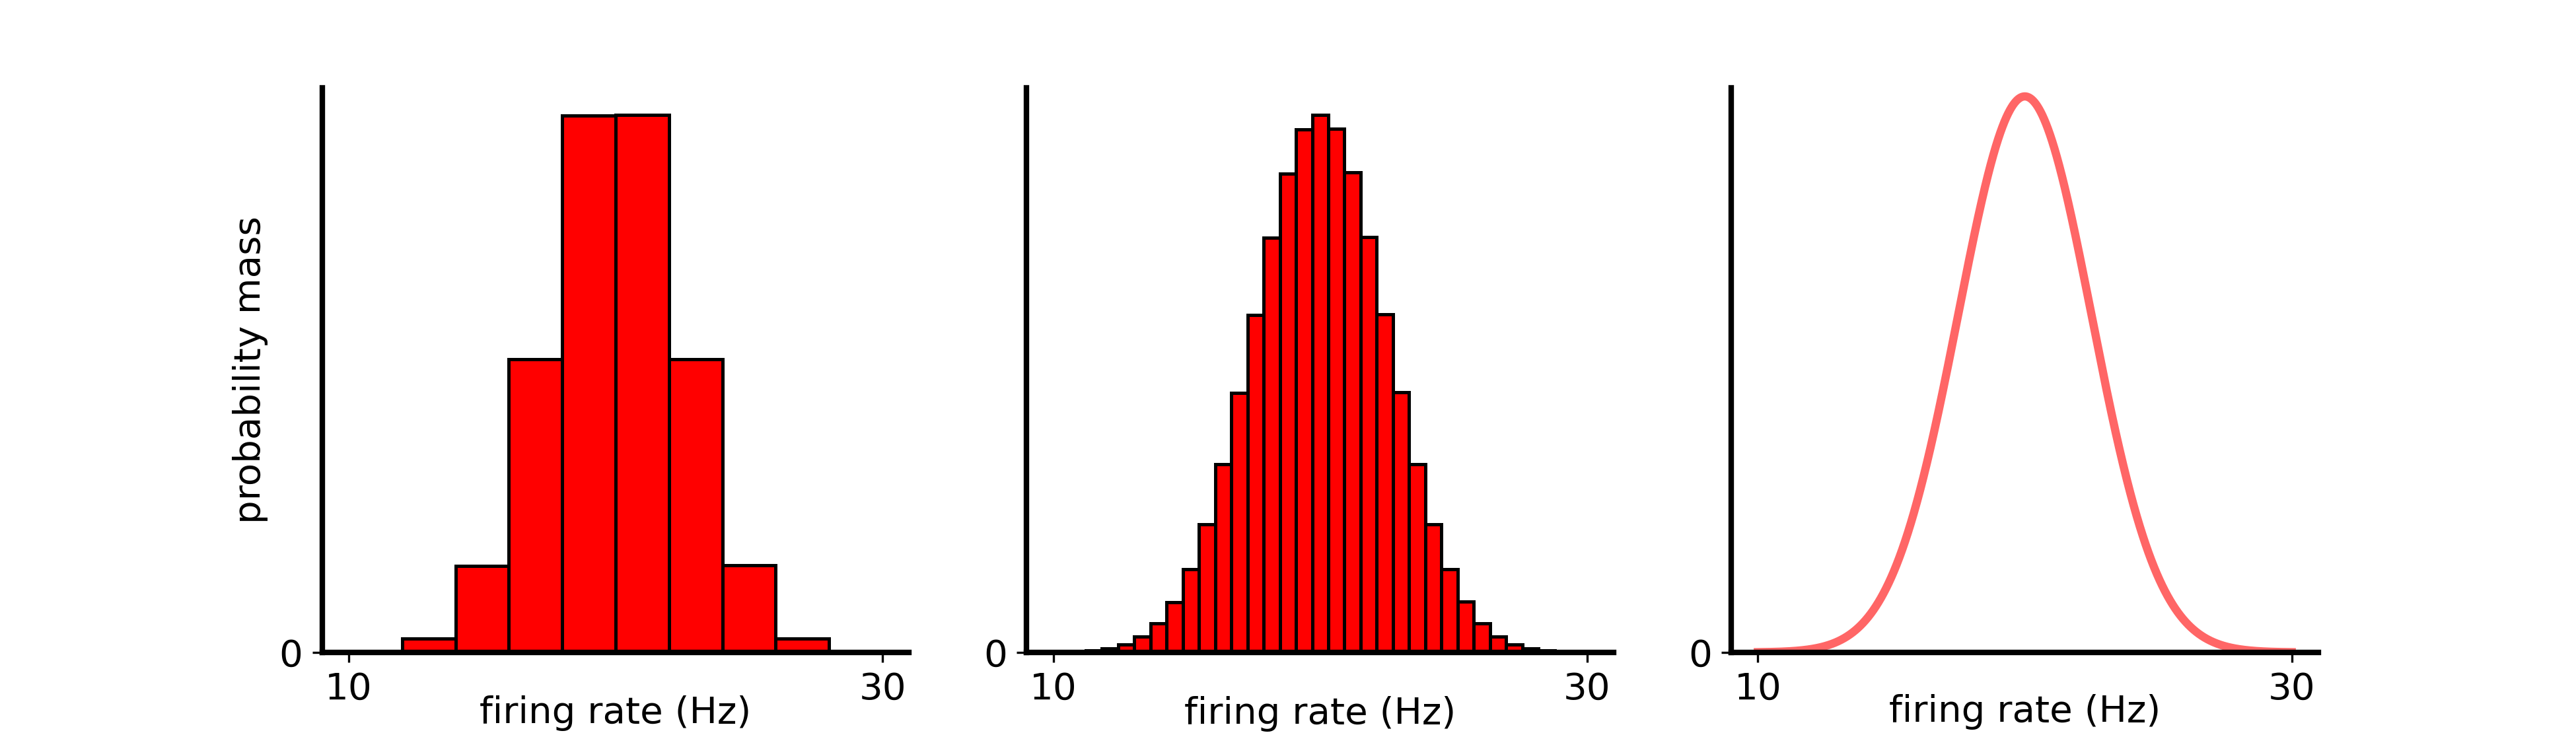
\includegraphics[height=2.5cm]{images/normal_mass_to_hist.png}
\vspace{-0.25cm}
\center 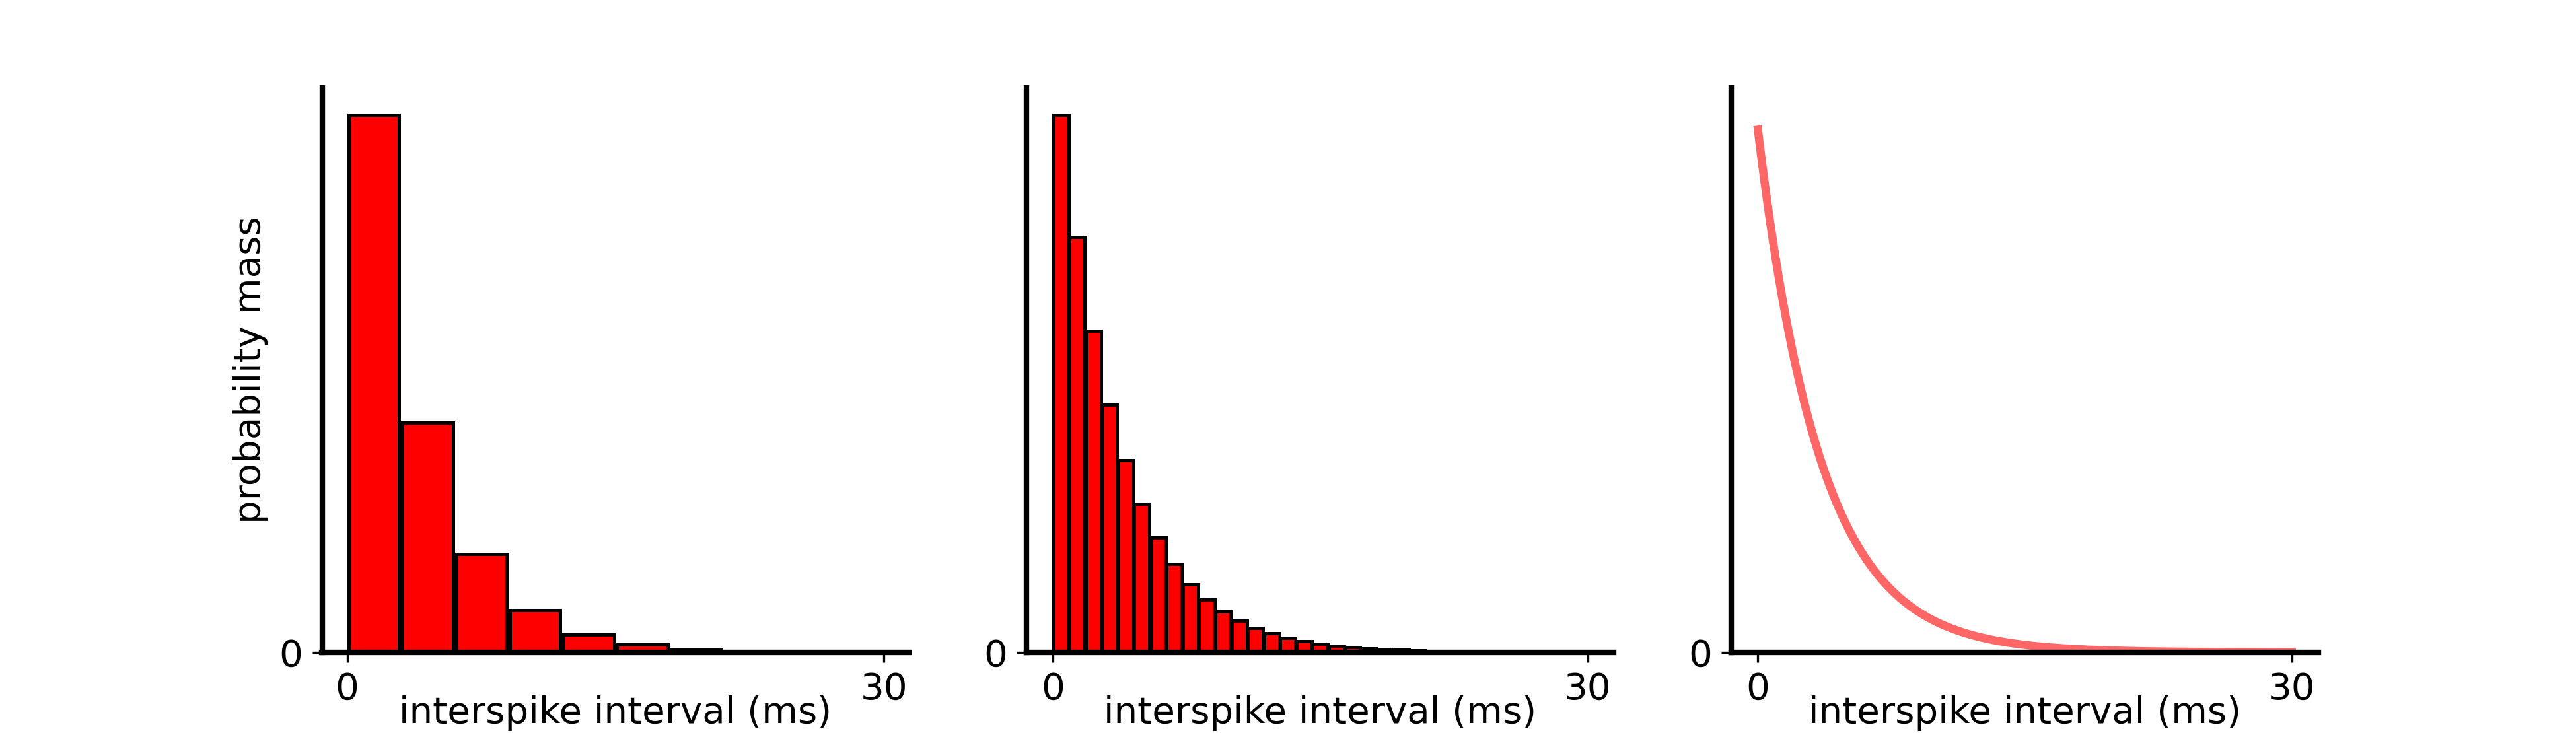
\includegraphics[height=2.5cm]{images/exp_mass_to_hist.png}

\end{frame}

%\begin{frame}
%\frametitle{Fly eye - normal stimulus distribution, CDF normal tuning curve}
%\vspace{-0.25cm}
%page 131 dayan aboot
%\end{frame}

%\begin{frame}
%\frametitle{Central Limit Theorem}
%\end{frame}

\begin{frame}
\frametitle{The probability density function}

\begin{definition} 
%A random variable $X$ is continuous if there exists a nonnegative function $f_X(x)$ defined on the interval $(-\infty, \infty)$, such that for any interval $[a, b]$ we have 
The \textbf{probability density function} (PDF) of a continuous random variable $X$ is a function $f_X(x)$ defined on the interval $(-\infty, \infty)$ such that for any two numbers $a$ and
$b$ with $a \leq b$,
\begin{equation*}
P(a \leq X \leq b) = \int_a^b f_X(x) dx.
\end{equation*} 
That is, the probability that $X$ takes on a value in the interval [a, b] is the area under the graph of the density function above this interval.
\end{definition}

\vspace{0.3cm}

\onslide<2->{
A valid probability density function $f_X(x)$ must have the following properties:

\begin{equation}
f_X(x) \geq 0 \text{ for all } x
\end{equation}

\begin{equation}
\int_{-\infty}^\infty f_X(x) dx = 1.
\end{equation}
}

\end{frame}

\begin{frame}
\frametitle{Probabilities as integrals}

The probability that a continuous random variable $X$ takes on a value in the interval [a, b] is given by the area under the probability density function $f_X(x)$:

\vspace{-0cm}

\begin{equation*}
P(a \leq X \leq b) = \int_a^b f_X(x) dx
\end{equation*}

\vspace{-0.2cm}
\begin{center}
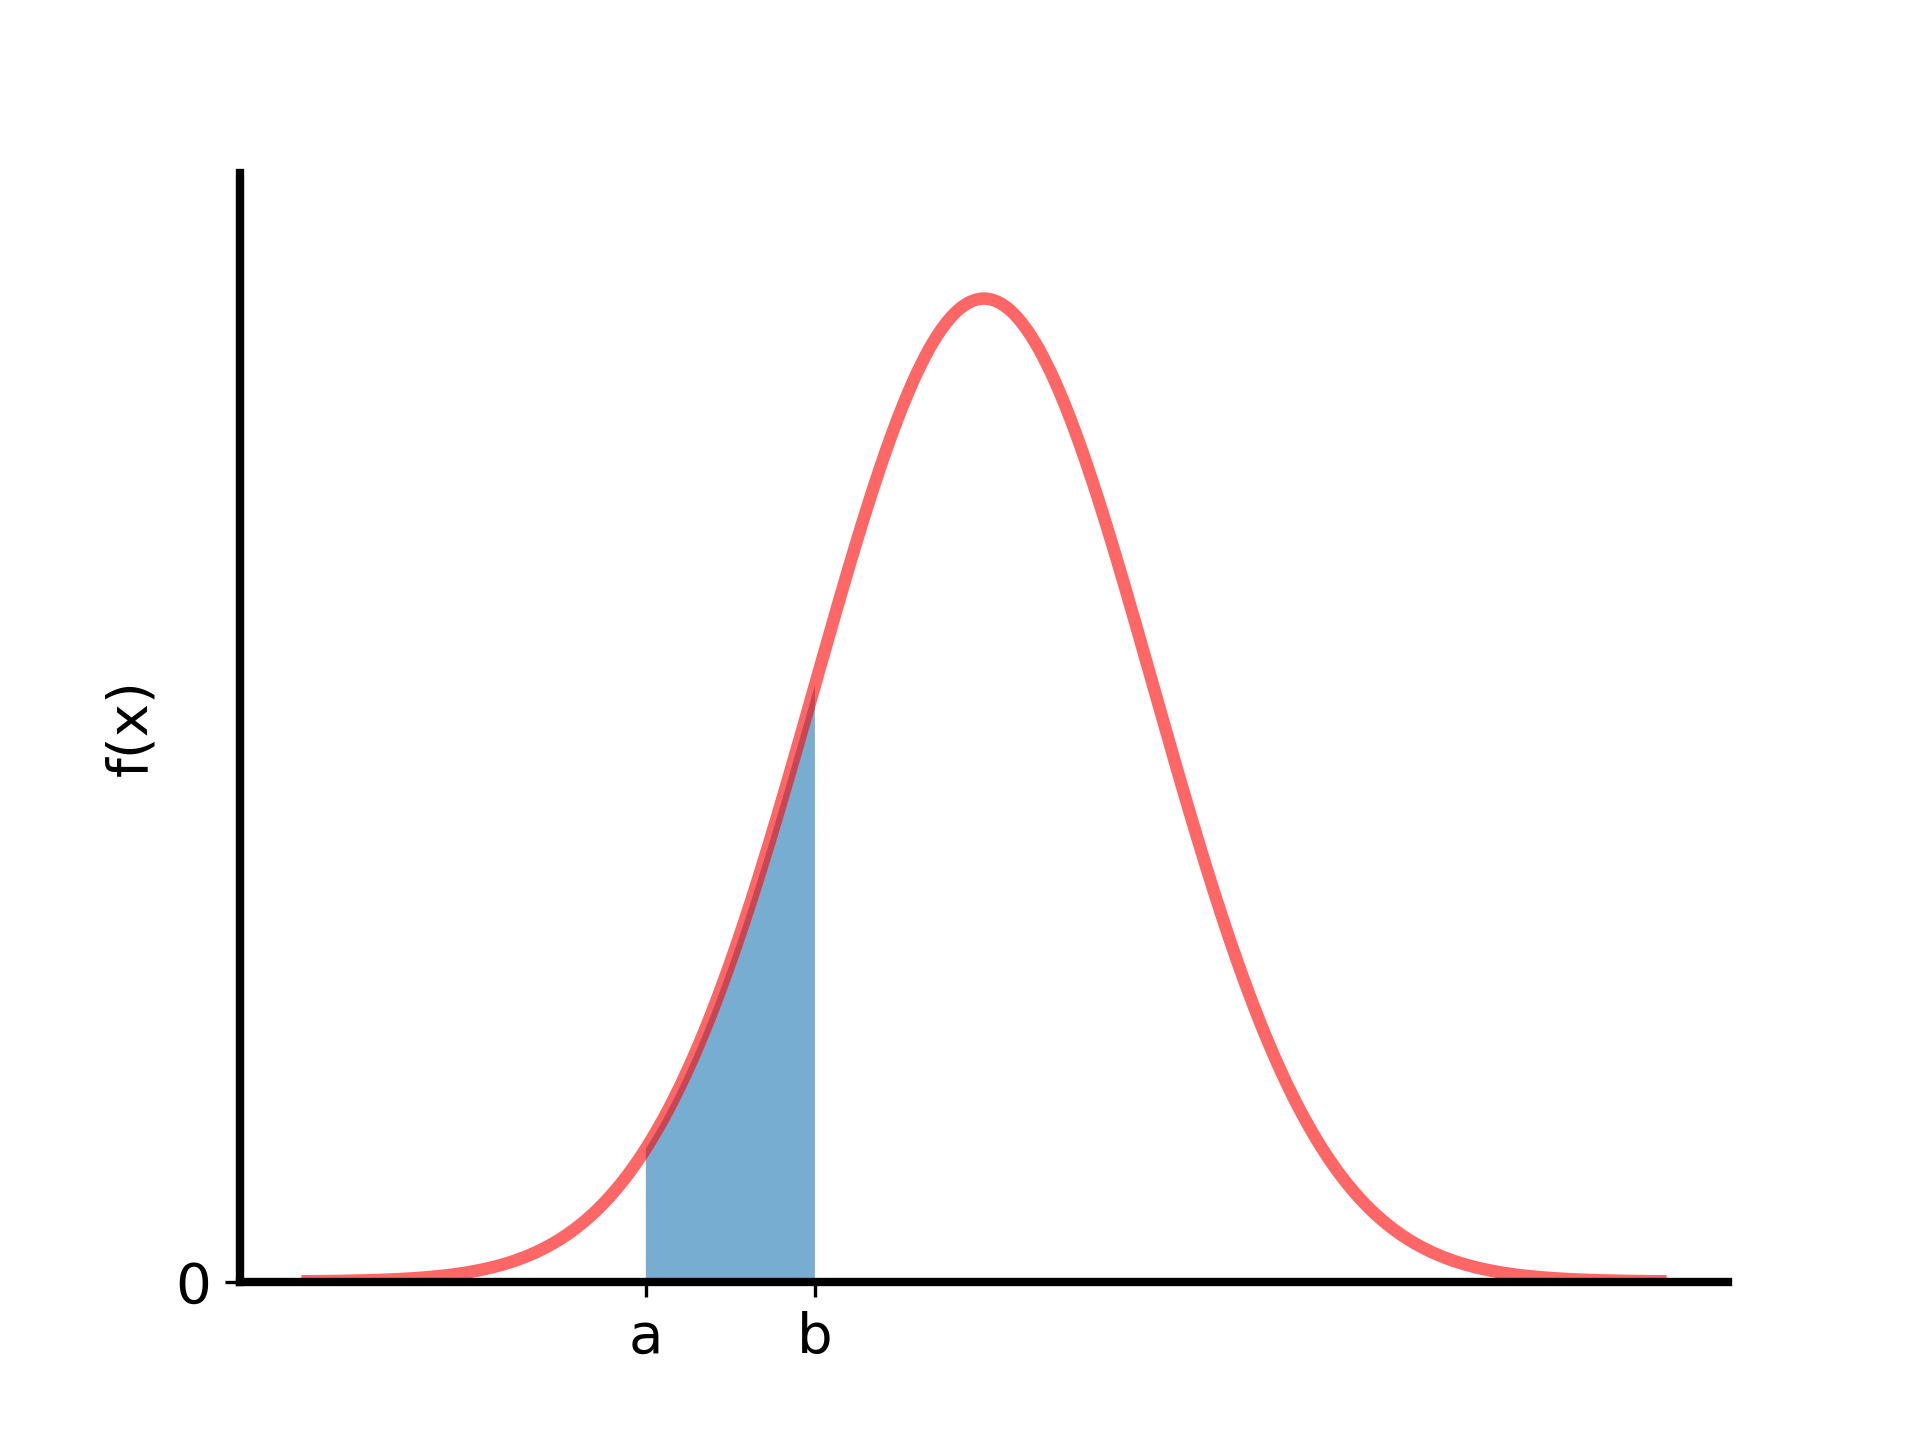
\includegraphics[height=3cm]{images/normal_area.png}
\end{center}

\end{frame}

\begin{frame}
\frametitle{Density as probability per unit of $x$}

If $f_X(x)$ is not the probability of $x$, what is it?

\

\onslide<2->{
The probability that $X$ will lie in an infinitesimal interval $dx$ about $x$ is
$f_X(x) dx$:

\vspace{-0.3cm}

\begin{align*}
P(x \leq X \leq x +dx) &= \int_x^{x+dx} f_X(t) dt\\
&= f_X(x) dx\\
\end{align*}
}

\vspace{-0.8cm}

\onslide<3->{
Thus, density is probability per unit of $x$ (rate of probability accumulation):

\begin{align*}
\frac{P(x \leq X \leq x + dx)}{dx} &= f_X(x) \ \ \ \ \ \ \ \ \ \ \ \
\end{align*} 
}

\end{frame}

% \begin{frame}
% \frametitle{Properties of the PDF}

% For a discrete random variable $X$, the probability mass function $p(X = x)$ satisfies:

% \begin{equation*}
% p(x) \geq 0 \textrm{ for all } x
% \end{equation*}

% \begin{equation*}
% \sum_x p(x) = 1
% \end{equation*}

% % NB these two proerties collectiveyl this implies p(x) leq to 1

% \end{frame}

\begin{frame}
\frametitle{Each possible value has zero probability}

The probability that $X$ takes on a particular value $a$ is 0, as 

\vspace{-0.25cm}

\begin{align*}
P(X = a) &= \int_a^a f_X(x) dx \\
&= \lim\limits_{\epsilon \to 0}  \int_{a-\epsilon}^{a+\epsilon} f_X(x) dx \\
&= 0.
\end{align*}

\onslide<2->{
This implies that probabilities don't depend on interval end points:

\vspace{-0.25cm}

\begin{align*}
P(a \leq X \leq b) = P(a < X < b) = P(a < X \leq b) = P(a \leq X < b),
\end{align*}

as  $P(X = a) = P(X = b) = 0$.
}

%\begin{theorem}
%$P(a \leq X \leq b) = P(a \leq X < b)$ because $P(X = b)$ = 0\\
%$P(a \leq X \leq b) = P(a < X \leq b)$ because $P(X = a)$ = 0\\
%$P(a \leq X \leq b) = P(a < X < b)$
%\end{theorem}

\end{frame}

\section{Cumulative distribution functions}
\begin{frame}
\frametitle{The cumulative distribution function}

The cumulative distribution function (CDF) $F_X(x)$ is the area under the probability density function $f_X(x)$ to the left of $x$.

\begin{center}
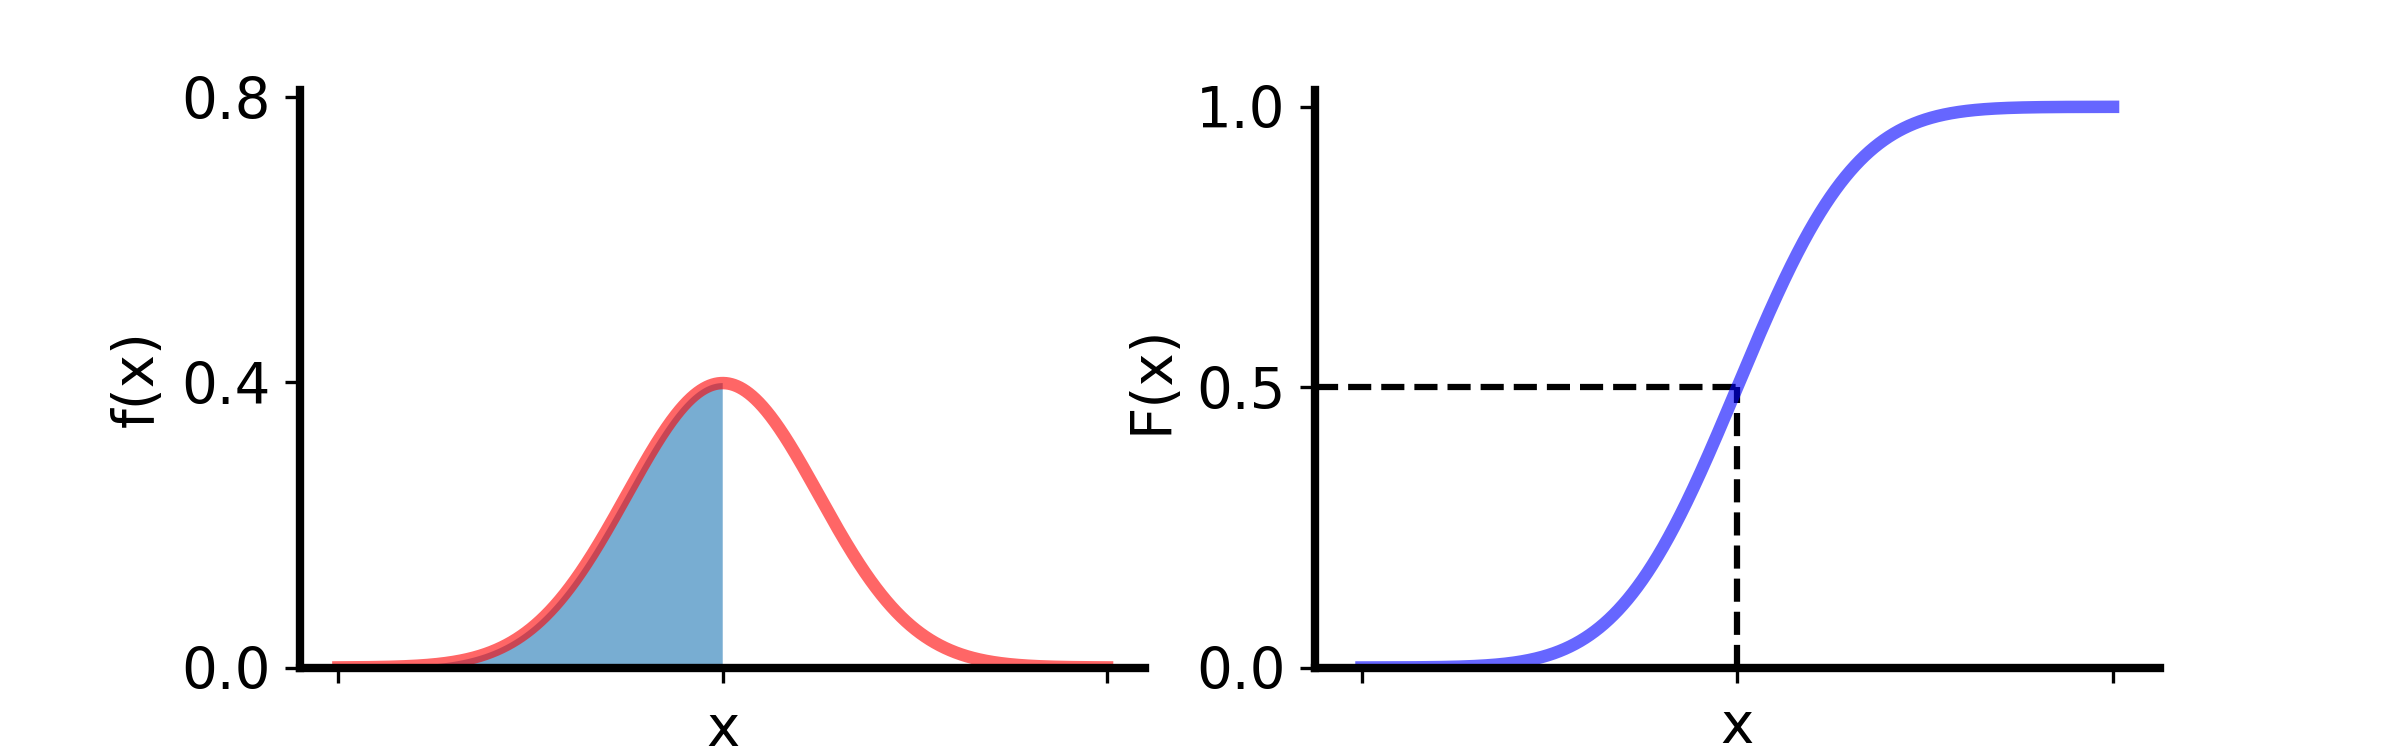
\includegraphics[height=2.5cm]{images/pdf_cdf_1.png}
\end{center}

\onslide<2->{
%The CDF is a non-decreasing (monotonic) function $F: \mathbb{R} \mapsto [0, 1]$ satisfying $\lim\limits_{x \to -\infty} F_X(x) = 0$ and $\lim\limits_{x \to \infty} F_X(x) = 1$.
The CDF $F_X(x)$ has the following properties:
\begin{enumerate}[label=\alph*.]
\item $F_X(x)$ is a non-decreasing (monotonic) function of $x$
\item $\lim\limits_{x \to -\infty} F_X(x) = 0$ and $\lim\limits_{x \to \infty} F_X(x) = 1$.
%\item $F_X(x)$ is right-continuous: $ \lim\limits_{\epsilon \to 0, \epsilon > 0}  F(x + \epsilon) = F_X(x)$ for any $x \in \mathbb{R}$.
\end{enumerate}
}

\

\onslide<3->{
Collectively, a. and b. imply that $F_X: \mathbb{R} \mapsto [0, 1]$.
}

\end{frame}

\begin{frame}
\frametitle{The cumulative distribution function}

%The cumulative distribution function $F_X(x)$ is the area under the probability density function to the left of x.

\vspace{.3cm}

\begin{definition} 
Let $X$ be a continuous random variable with probability density function $f_X(x)$, then the \textbf{cumulative distribution function} $F_X(x)$ is defined as
\begin{align*}
F_X(x) &= P(X \leq x)\\
&= \int_{-\infty}^x f_X(t) dt.
\end{align*} 
\end{definition}

\vspace{0.5cm}


\end{frame}

\begin{frame}
\frametitle{Computing probabilities using the CDF}

% The cumulative distribution function encodes probabilities

%For any two numbers $a$ and $b$ with $a < b$,

\vspace{-.7cm}

\begin{align*}
P(a \leq X \leq b) = F_X(b) - F_X(a).
\end{align*} 

%\vspace{-1cm}

\vspace{-.4cm}

\center 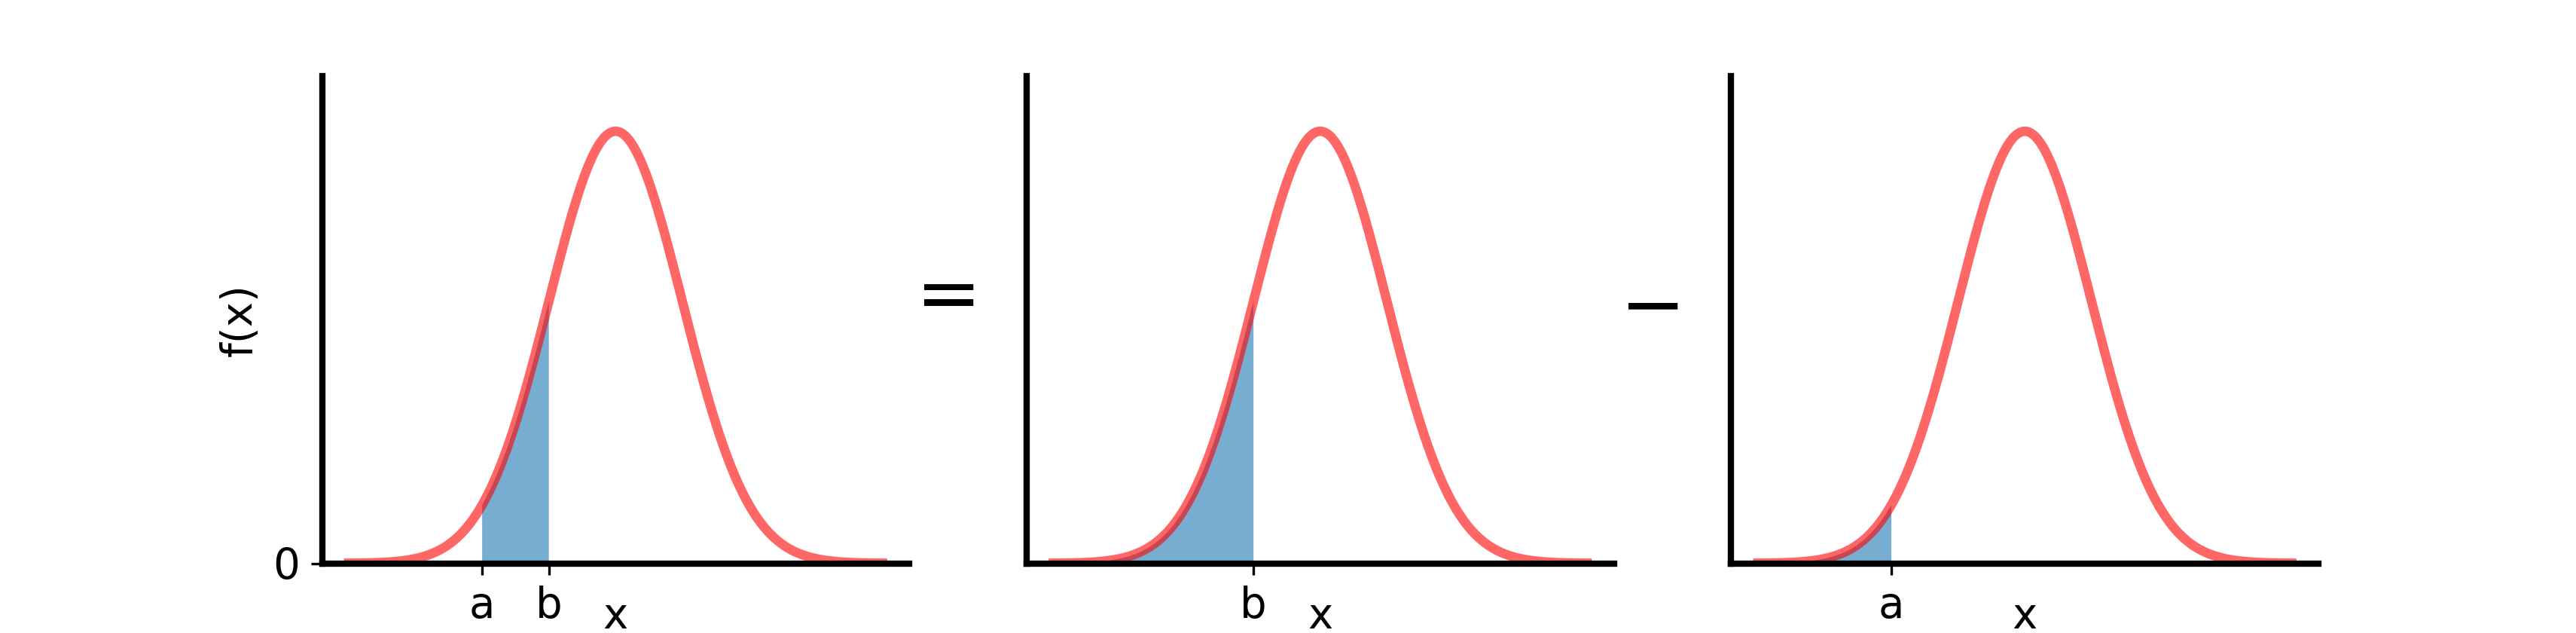
\includegraphics[height=2.5cm]{images/normal_ab_a_b.png}

\vspace{0cm}

%%For any number $a$,

\onslide<2->{
\begin{align*}
P(X > a) &= F_X(\infty) - F_X(a)\\
&= 1 - F_X(a).
\end{align*} 

\vspace{-.5cm}

\center 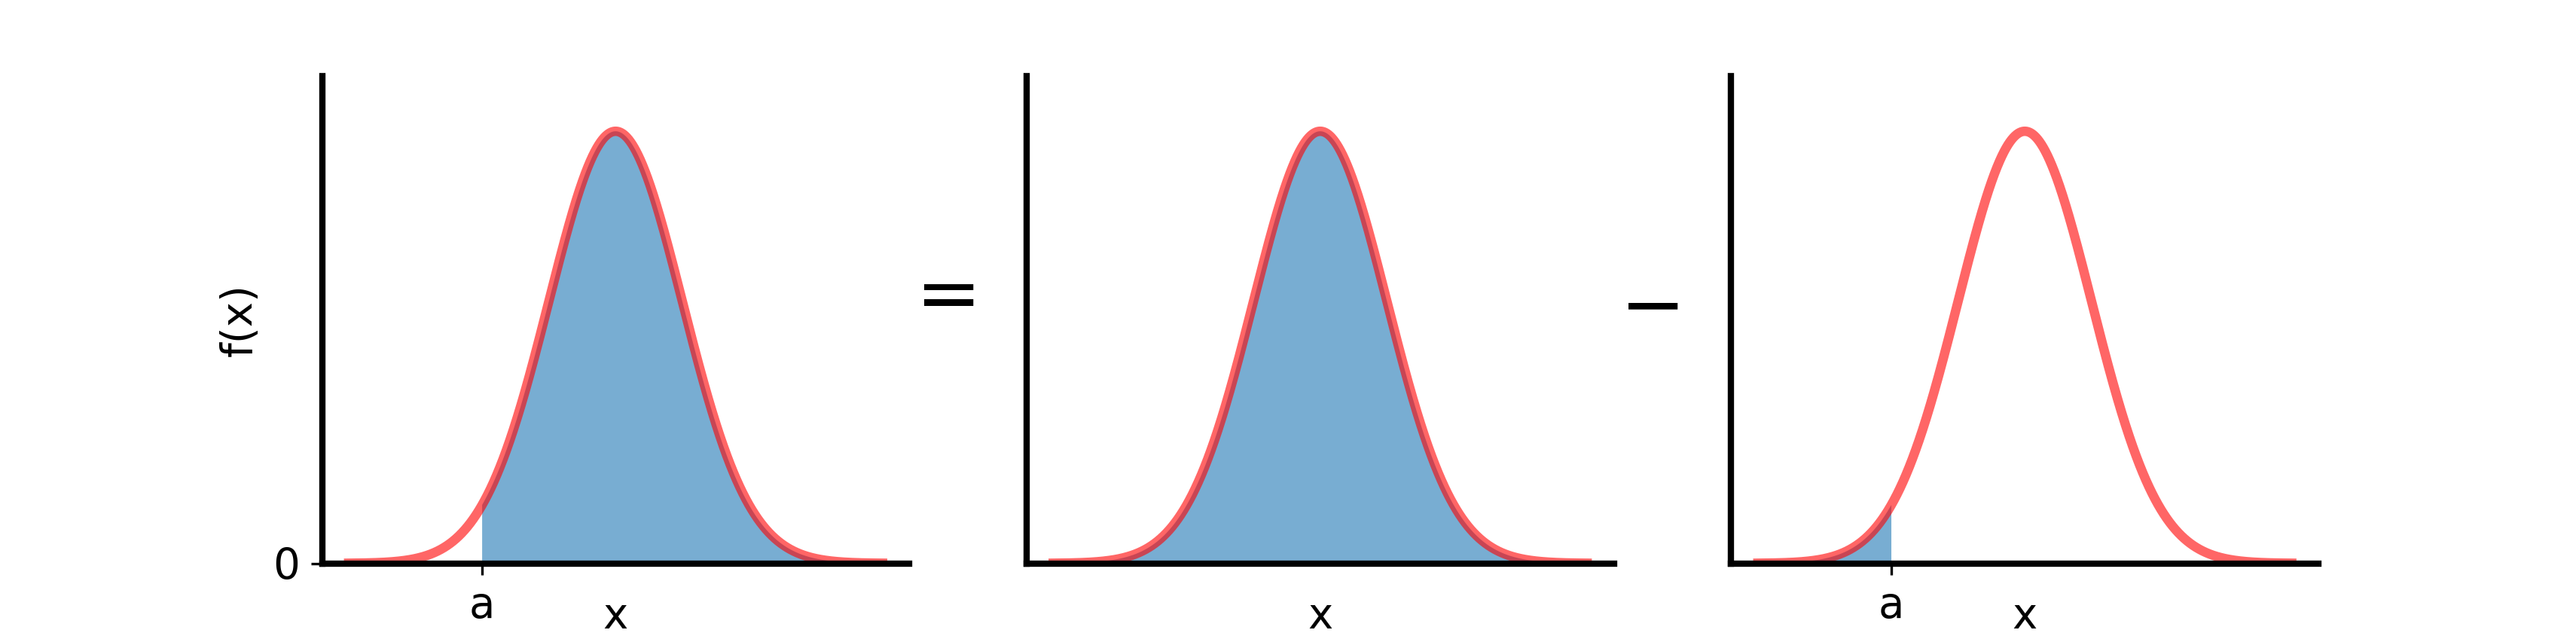
\includegraphics[height=2.5cm]{images/normal_a_inf.png}
}


%\begin{theorem}
%$P(a \leq X \leq b) = F(b) - F(a)$
%\end{theorem}
%
%\begin{proof}
%% $P(a \leq X \leq b) = P(X \leq b) - P(X < a)$\\0
%% But because $X$ is continuous, $P(X < a) = P(X \leq a)$, and so
%\begin{align*}
%P(a \leq X \leq b) &= P(X \leq b) - P(X < a)\\
%&= P(X \leq b) - P(X \leq a)\\
%&= F(b) - F(a)
%\end{align*} 
%\end{proof}

\end{frame}

\begin{frame}
\frametitle{Obtaining the PDF from the CDF}

How would you obtain the PDF from the CDF?

\

\onslide<2->{
The CDF is the integral of the PDF, and so the PDF is the derivative of the CDF.
}

\onslide<3->{
\begin{center} 
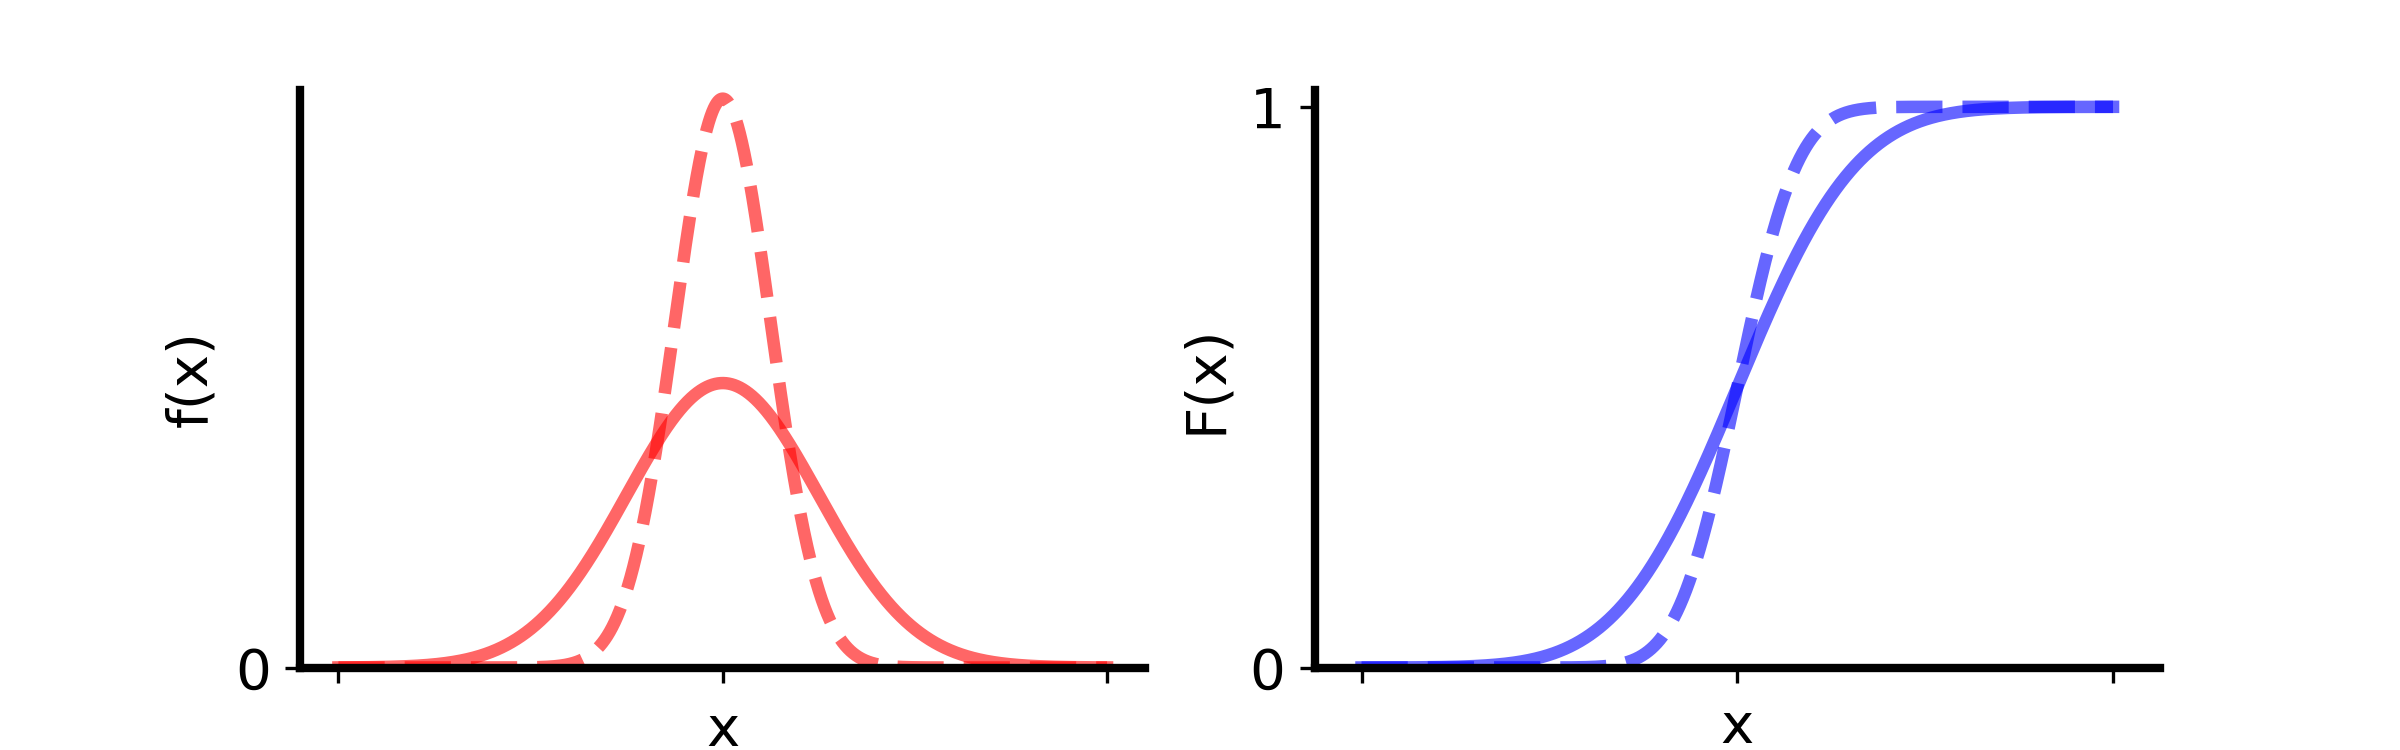
\includegraphics[height=2.5cm]{images/pdf_cdf_nofill.png}
\end{center} 
}

\

%At every $x$ at which the derivative $F^\prime(x)$ exists, $F^\prime(x) = f_X(x)$.
%At every $x$ at which the derivative $\frac{\delta F_X(x)}{\delta x}$ exists, $\frac{\delta F_X(x)}{\delta x} = f_X(x)$.
\onslide<4->{
At every $x$ at which the derivative $\frac{\delta F_X(x)}{\delta x}$ exists, $\frac{\delta F_X(x)}{\delta x} = f_X(x)$.
}

\end{frame}

\begin{frame}
\frametitle{Example: the uniform distribution}

\vspace{-.05cm}

\begin{definition}
A continuous random variable $X$ is said to have a \textbf{uniform distribution} on the interval ${[a, b]}$ if the PDF of $X$ is

\vspace{-.5cm}

\begin{align*}
    f_X(x; a, b) &= 
    \begin{cases}
      \frac{1}{b-a} & \text{if}\ a \leq x \leq b \\
      0 & \text{otherwise,}
    \end{cases}
\end{align*}
and the CDF of $X$ is
\begin{align*}
F_X(x; a, b) &= 
    \begin{cases}
      0 & \text{if}\ x < a \\
      \frac{x-a}{b-a} & \text{if}\ a \leq x \leq b \\
      1 &\text{if}\ x > b. \\
    \end{cases}
\end{align*}
When $X$ has a uniform distribution on [$a, b$], we write this as $X \sim \U{a,b}$. 
\end{definition}

%\center 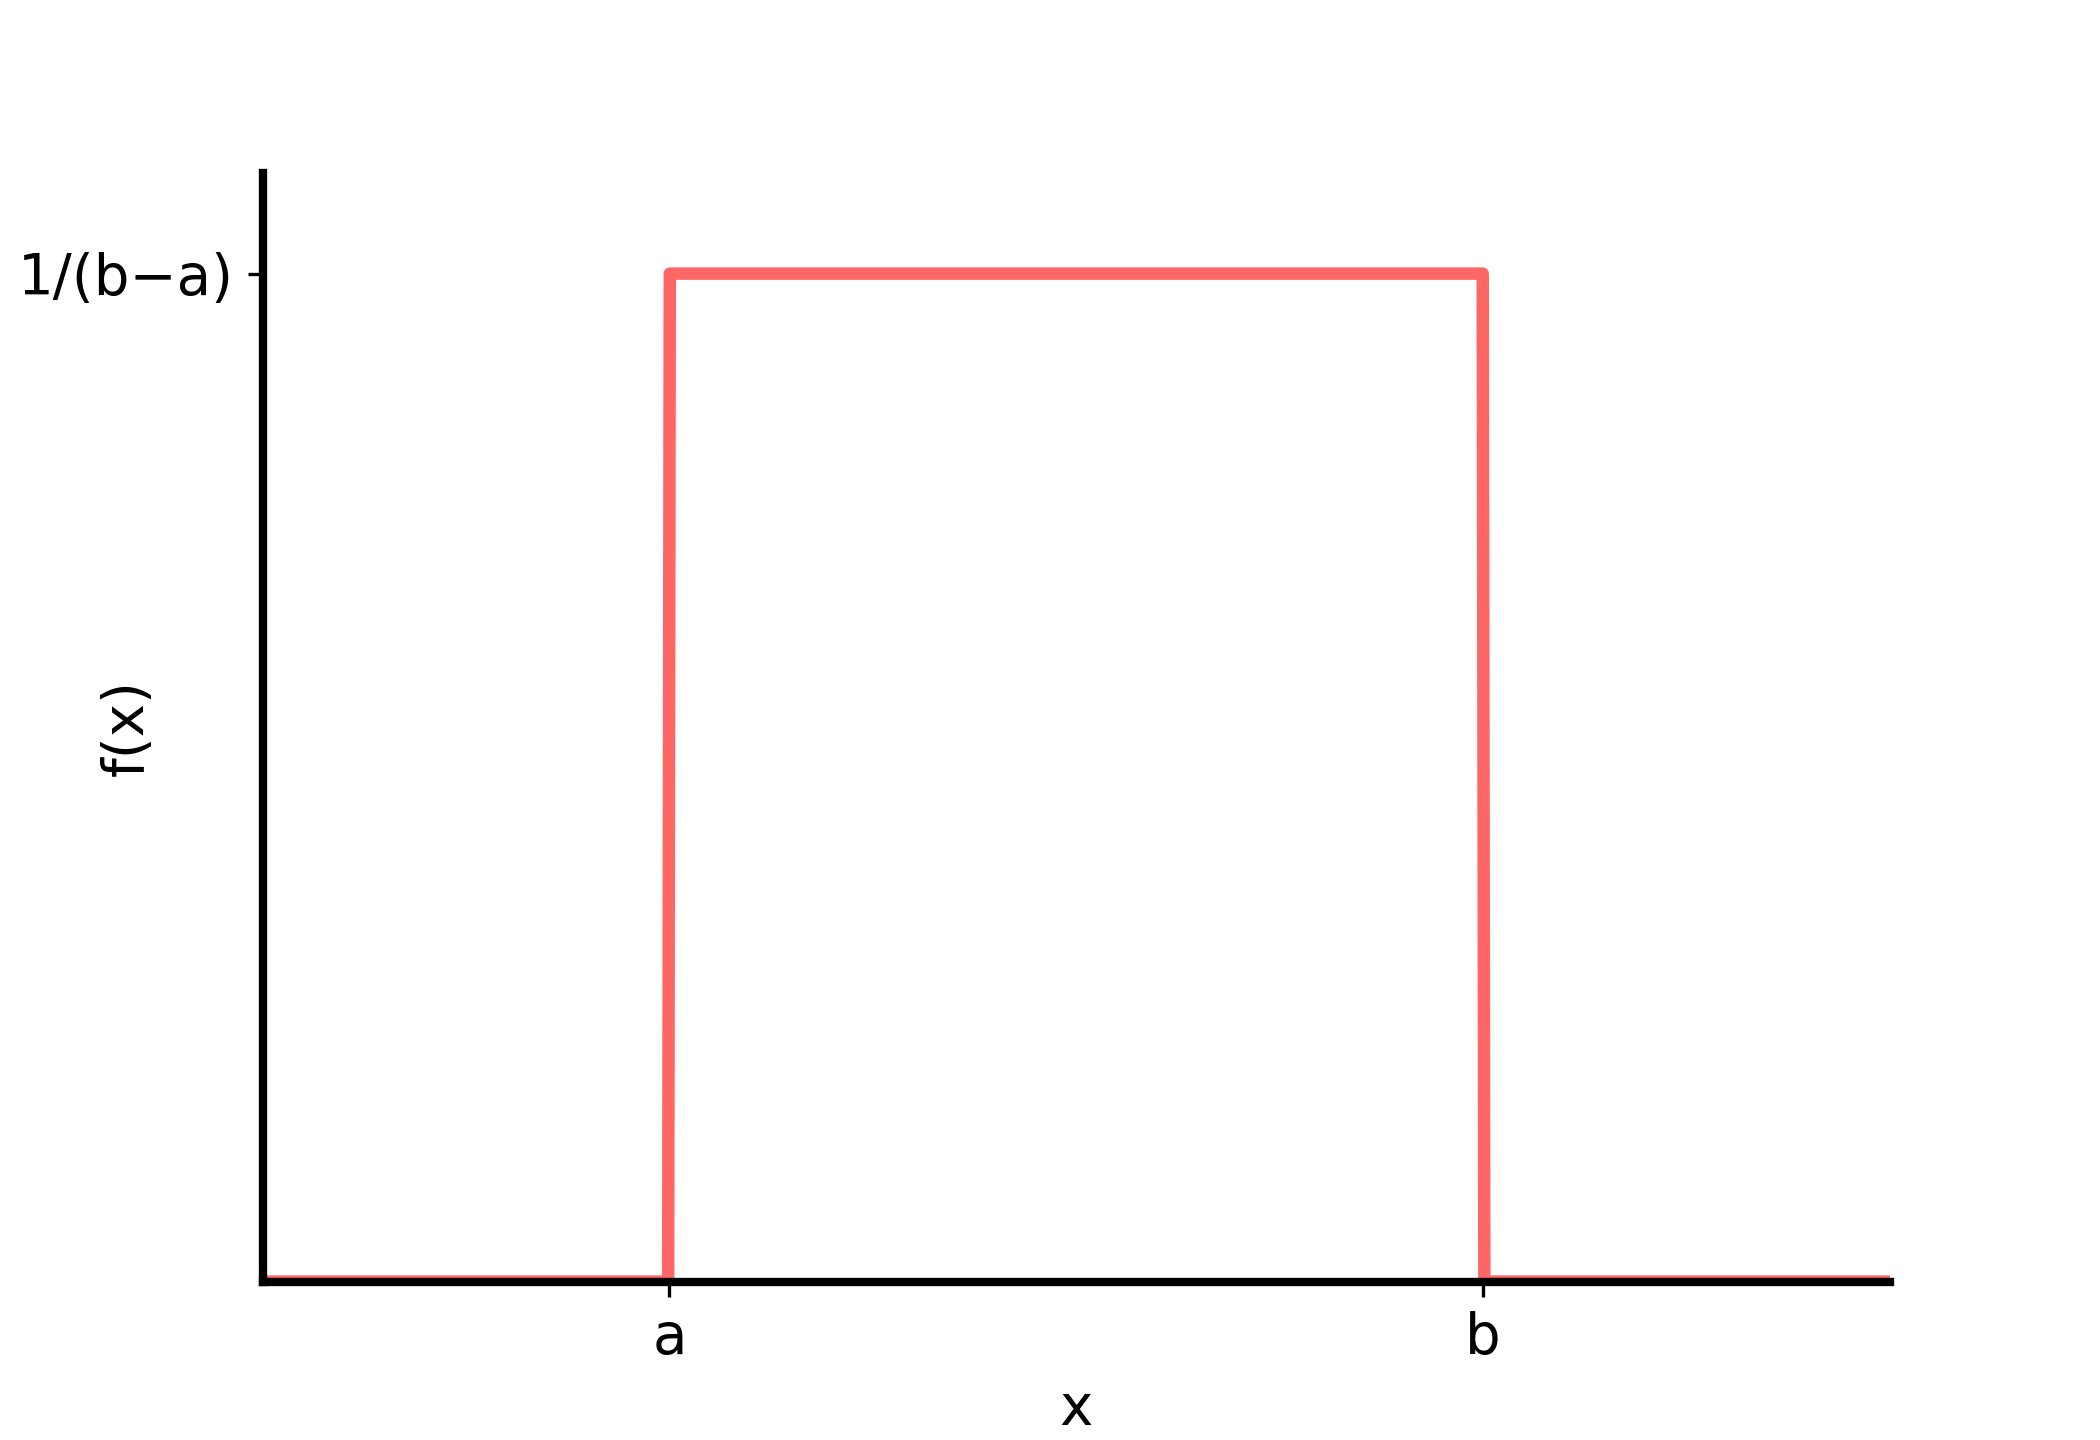
\includegraphics[height=3.6cm]{images/uniform_pdf.png}

\onslide<2->{
\begin{example}
When $X \sim \U{a,b}$, for $a \leq x \leq b$:

\vspace{-0.3cm}

\begin{align*}
%F^\prime(x) = \frac{d}{dx}\bigg(\frac{x-a}{b-a}\bigg) = \frac{1}{b-a} = f_X(x)
\frac{\delta F_X(x)}{\delta x} = \frac{\delta}{\delta x}\bigg(\frac{x-a}{b-a}\bigg) = \frac{1}{b-a} = f_X(x)
\end{align*}
\end{example}
}
%F_X(x) is differentiable except at and where the graph of F_X(x) has sharp corners.

\

\end{frame}

\begin{frame}
\frametitle{Percentiles of a continuous distribution}

\begin{definition}
Let $p$ be a number between 0 and 1. The \textbf{(100$p$)th percentile} of the distribution
of a continuous random variable $X$, denoted by $\eta(p)$, is defined by
\begin{align*}
p = F_X(\eta(p)) = \int_{-\infty}^{\eta(p)}f_X(x) dx
\end{align*}
\end{definition}

\onslide<2->{
\center 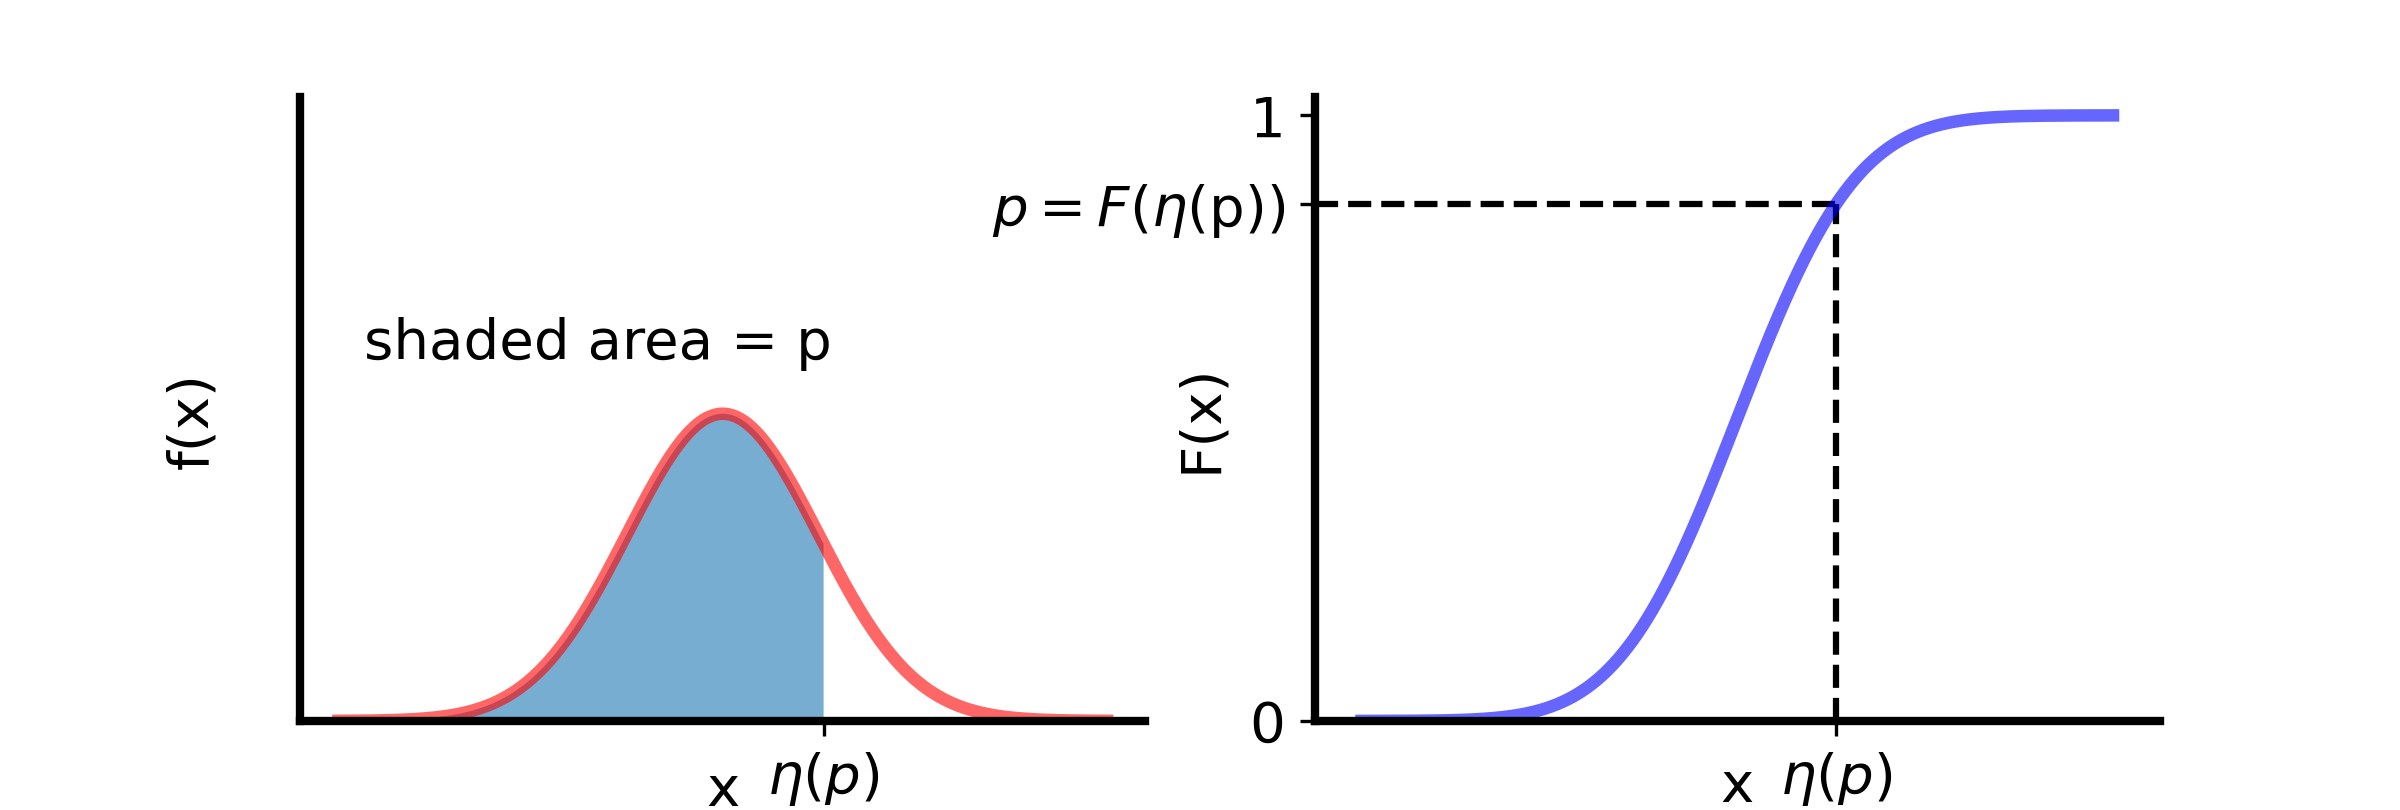
\includegraphics[height=3cm]{images/percentiles.png}
}

\end{frame}

\begin{frame}
\frametitle{Median}

\begin{definition}
The \textbf{median} of a continuous distribution, denoted by $\tilde{\mu}$, is the 50th percentile, so $\tilde{\mu}$ satisfies $F_X( \tilde{\mu}) = 0.5$. That is, half the are area under the probability density function is to the left of $\tilde{\mu}$ and half is to the right of $\tilde{\mu}$.
\end{definition}

\center 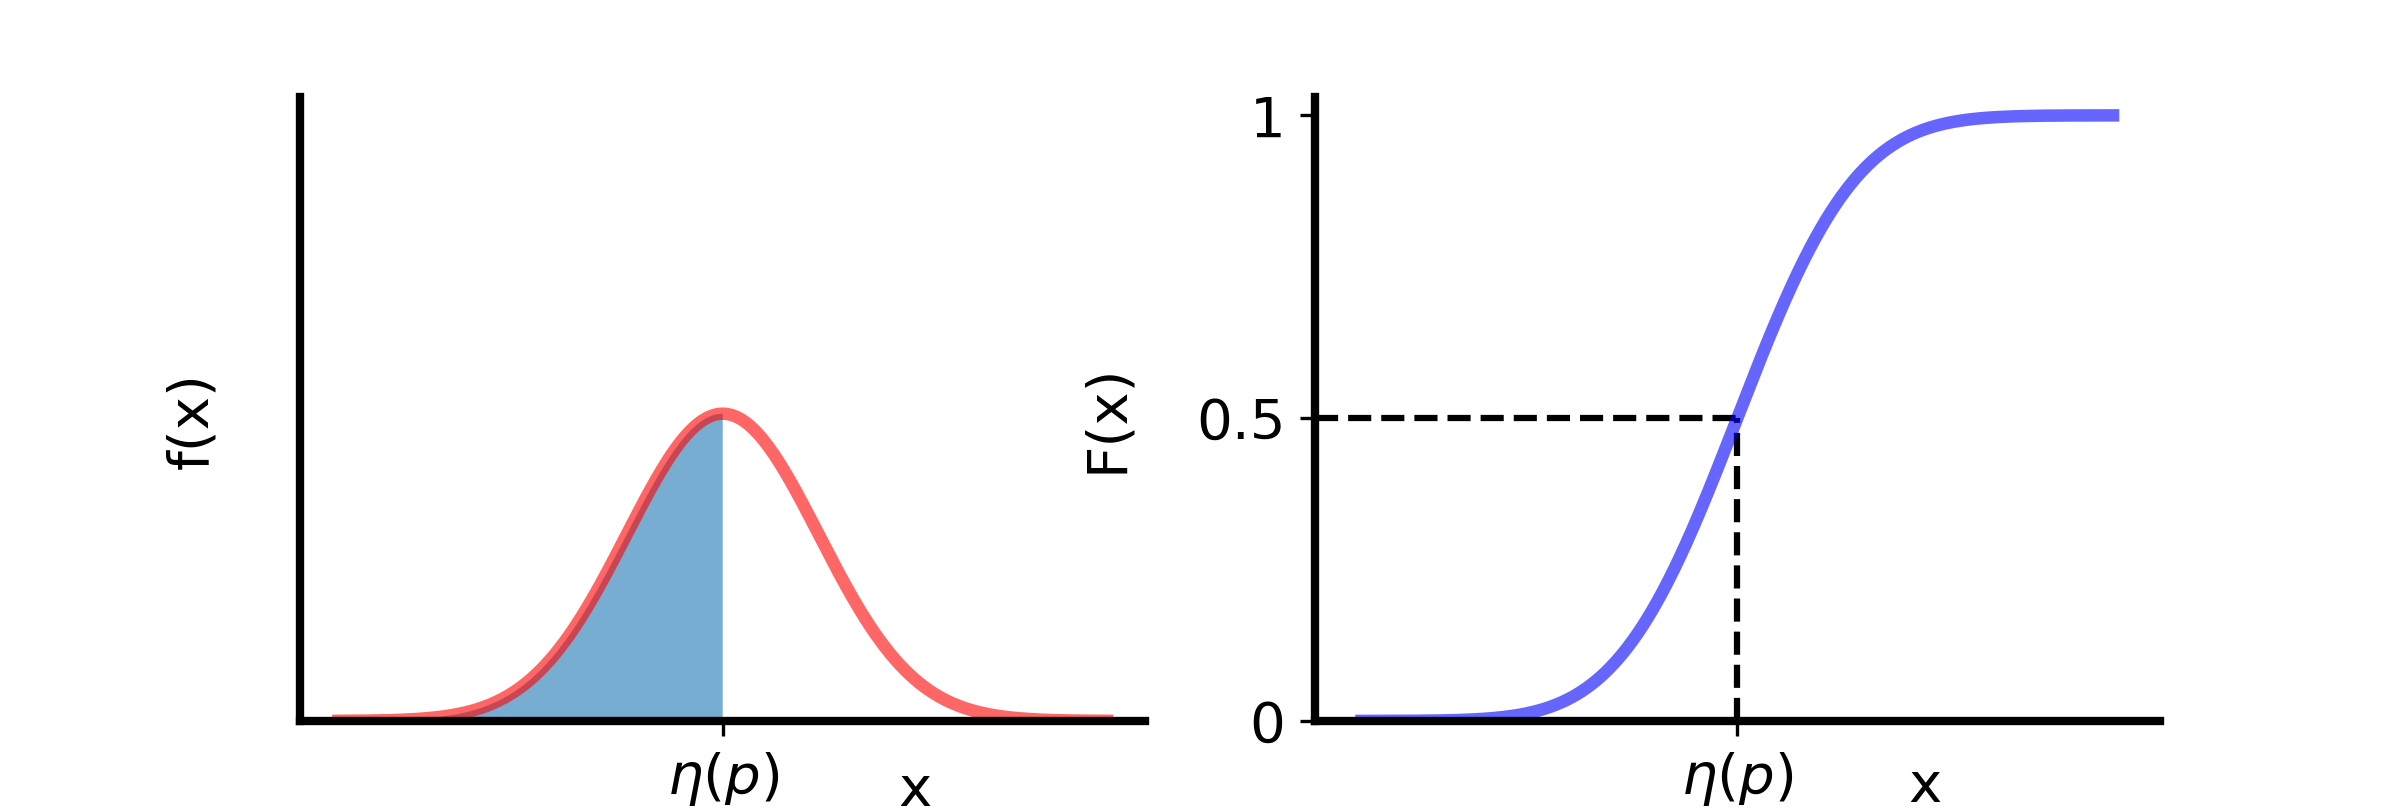
\includegraphics[height=3cm]{images/median.png}

\end{frame}

\begin{frame}
\frametitle{Example: the exponential distribution}

\begin{definition}
A random variable $X$ is said to have an \textbf{exponential distribution} on the interval [0, $\infty$) if the PDF of $X$ is:

\vspace{-.5cm}

\begin{align*}
    f_X(x; \lambda) &= 
    \begin{cases}
      \lambda e ^{-\lambda x} & \text{if}\ x \geq 0 \\
      0 & \text{otherwise},
    \end{cases}
\end{align*}
where $\lambda > 0$ is a rate parameter that governs the rate of decay of $f_X(x)$. When $X$ has an exponential distribution with parameter $\lambda$, we write $X \sim \Exp{\lambda}$. 
\end{definition}

\center 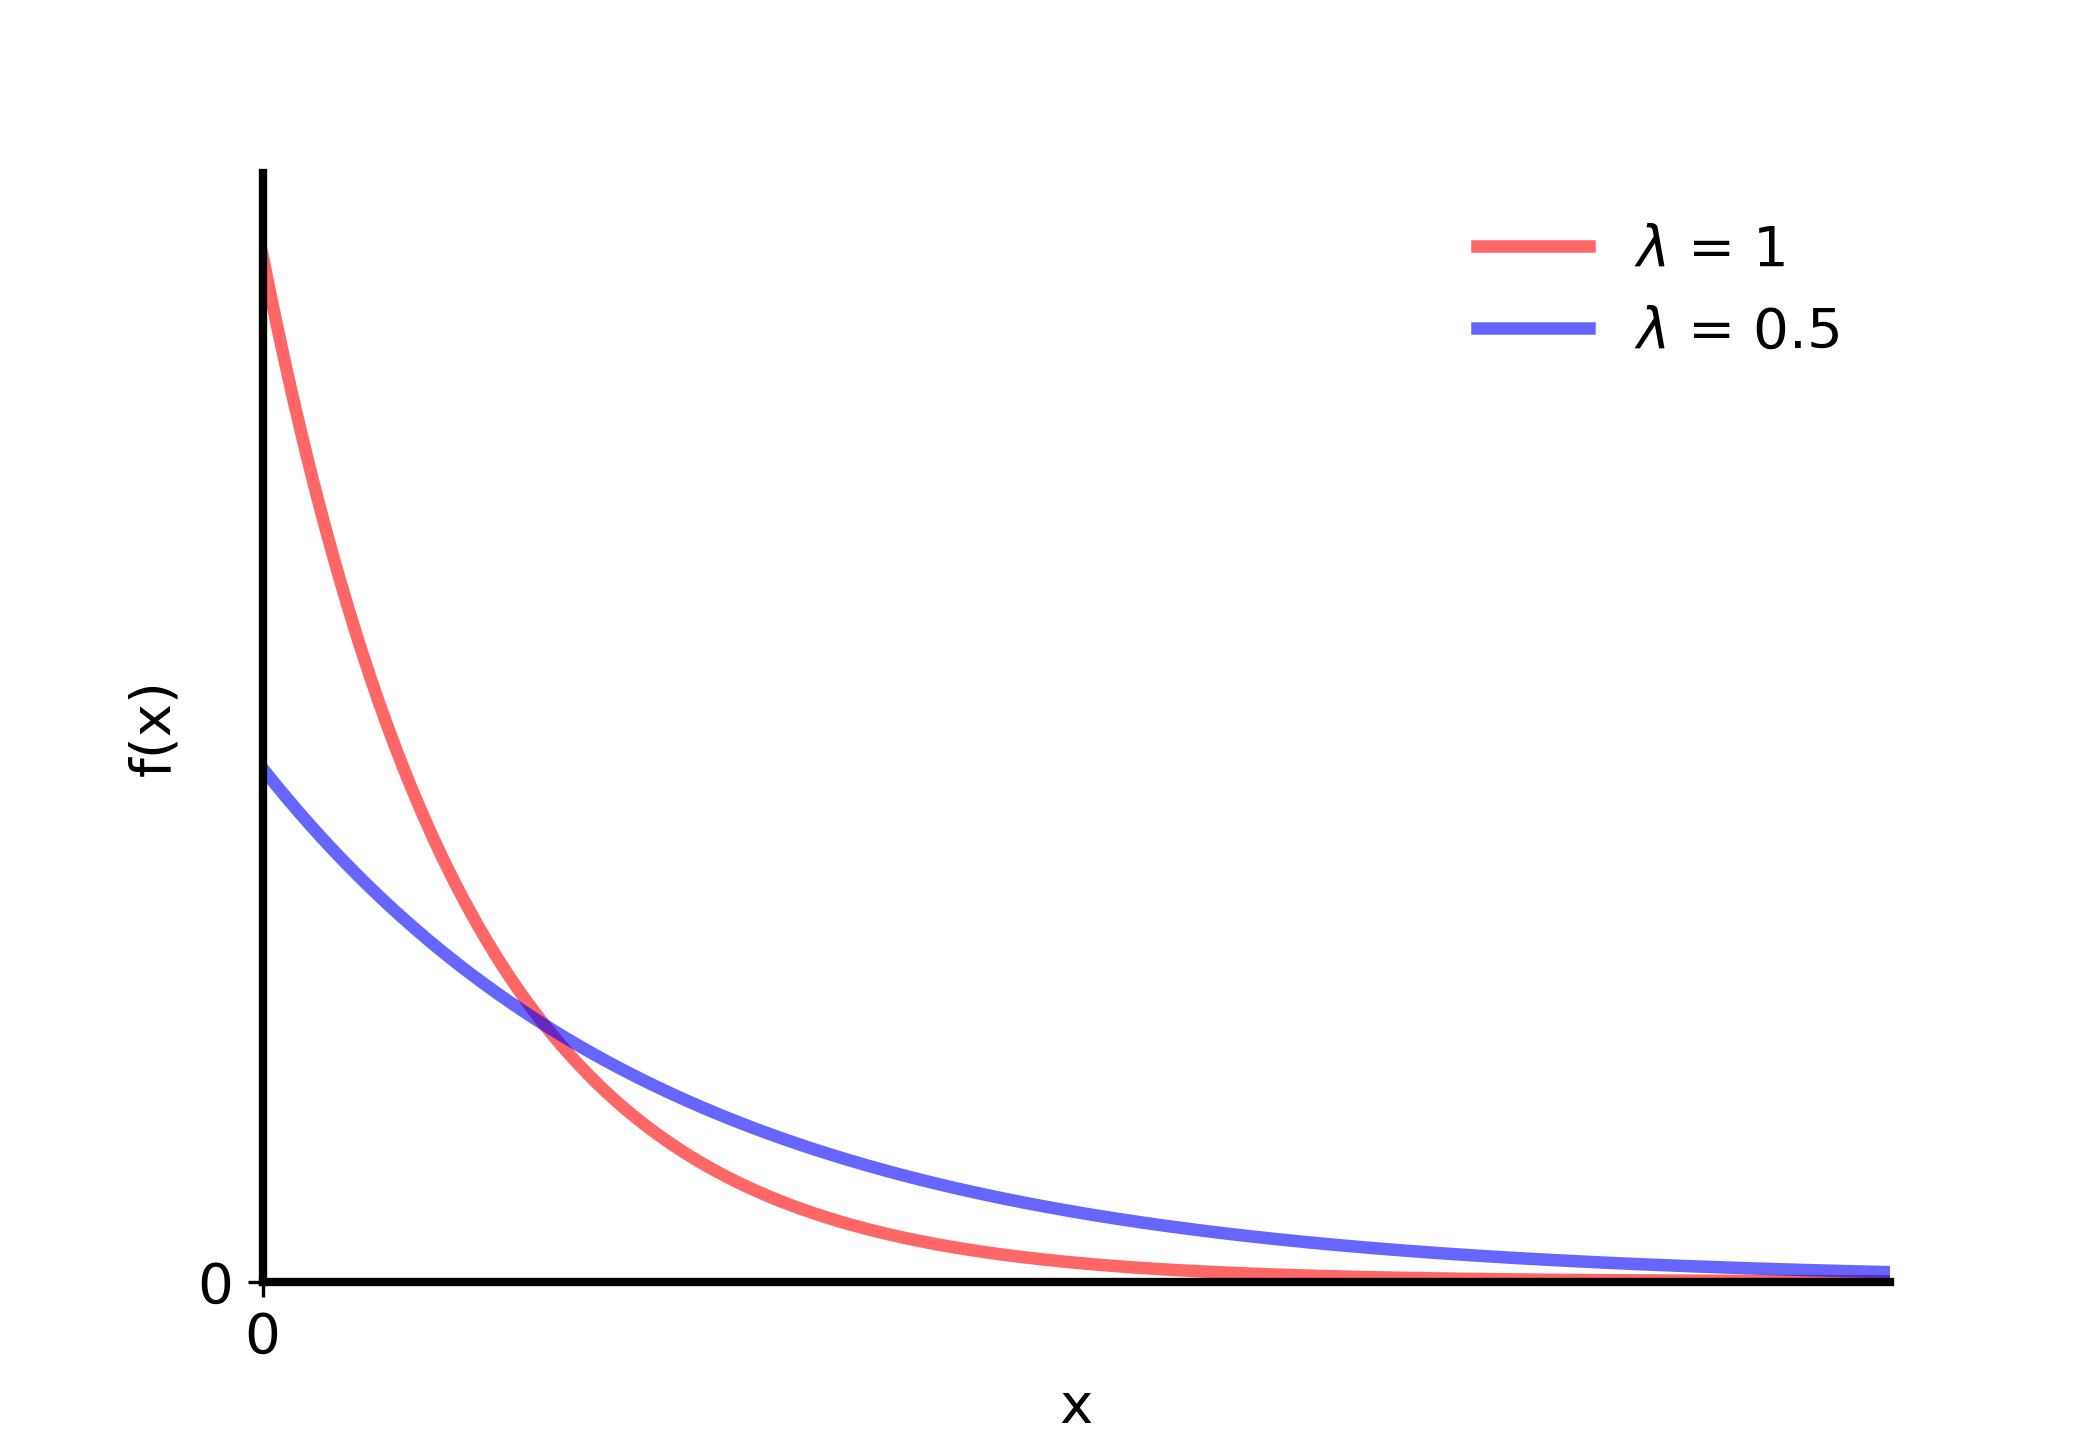
\includegraphics[height=3cm]{images/exp_pdf.png}

\end{frame}

\begin{frame}
\frametitle{Example: the exponential distribution}

\begin{example}
Write down the formula for the (100$p$)th percentile of the distribution of $X \sim \Exp{\lambda}$, and use it to find the median of $X$.
\begin{align*}
\onslide<2->{
p &= \int^{\eta(p)}_0 \lambda e^{-\lambda x}dx\\
}
\onslide<3->{
&=  - e^{-\lambda x}\Big|_0^{\eta(p)}\\
}
\onslide<4->{
&=  1 - e^{-\lambda \eta(p)}.
}
\onslide<5->{
\intertext{Therefore,}
\eta(p) &=  -\frac{\log{(1 - p)}}{\lambda}
}
\onslide<6->{
\intertext{and}
\eta(0.5) &=  -\frac{\log{(0.5)}}{\lambda}.
}
 \end{align*}
 
\end{example}

\end{frame}

\section{Expected values}
\begin{frame}
\frametitle{Expected value of a function of a continuous random variable}

The expected value (mean) of a continuous random variable $X$ is:

\begin{equation*}
\mathbb{E}[X] = \int_{-\infty}^\infty x f_X(x) dx.
\end{equation*}

\vspace{.1cm}

\onslide<2->{
The expected value of a function $g(x)$ of $X$ is:

\begin{equation*}
\mathbb{E}[g(X)] = \int_{-\infty}^\infty g(x) f_X(x) dx.
\end{equation*}
}

\onslide<3->{
The variance of $X$ is:

\vspace{-.4cm}

\begin{align*}
% var[X] &= \mathbb{E}[(X - \mathbb{E}[X])^2]\\
\mathrm{Var}[X] &= \int_{-\infty}^\infty (x - \mathbb{E}[X])^2 f_X(x) dx\\
&= \mathbb{E}[(x - \mathbb{E}[X])^2] \\
&= \mathbb{E}[X^2] - \mathbb{E}[X]^2.
\end{align*}
}
% var[X] is an example of g(x)

% \begin{equation}
% var[X] = \mathbb{E}[X^2] - \mathbb{E}[X]^2
% \end{equation}

% \begin{equation}
% \mathbb{E}[X^2] = \int_{-\infty}^\infty x^2 f_X(x) dx
% \end{equation}

% Mode

\end{frame}

\begin{frame}
\frametitle{Example: the uniform distribution}

\begin{example}
When $X \sim \U{a,b}$, the expected value of $X$ is:

\vspace{-.3cm}

\begin{align*}
    \mathbb{E}[X] &= \int_{a}^b x \frac{1}{b-a} dx \\% \int_{-\infty}^\infty x f_X(x) dx \\
    \onslide<2->{
    &= \frac{b^2 - a^2}{2(b-a)}\\
    }
    \onslide<3->{
    &= \frac{a + b}{2},
    }
\end{align*}

\onslide<4->{
and the variance of $X$ is:

\vspace{-.3cm}

\begin{align*}
    \mathrm{Var}[X] &= \int_a^b x^2 \frac{1}{b-a} dx - \bigg( \frac{a + b}{2}\bigg)^2\\ % \int_{-\infty}^\infty (x - \mathbb{E}[X])^2 f_X(x) dx\\
    }
    \onslide<5->{
    &= \frac{b^3 - a^3}{3(b-a)} - \bigg( \frac{a + b}{2}\bigg)^2\\
    }
    \onslide<6->{
    &= \frac{(b-a)^2}{12}.
    }
\end{align*}

\end{example}

\end{frame}

%\section{Sampling}
%\begin{frame}
%\frametitle{The inverse transform method}
%
%\begin{theorem}
%Let $U \sim \U{0,1}$ be a continuous random variable having a standard uniform distribution on the interval [0,1]. Then, the random variable
%\begin{equation*}
%X = F^{-1}(U)
%\end{equation*}
%is distributed as the cumulative distribution function $F$, that is $P(X \leq x) = F_X(x)$.
%\end{theorem}
%
%\onslide<2->{
%\begin{proof}
%\begin{equation*}
%\begin{aligned}
%P(X \leq x) &= P(F^{-1}(U) \leq x)\\
%}
%\onslide<3->{
%&= P(F(F^{-1}(U)) \leq F_X(x)) \\
%}
%\onslide<4->{
%&= P(U \leq F_X(x)) \\
%}
%\onslide<5->{
%&= F_X(x).\qedhere
%\end{aligned} 
%\end{equation*}
%\text{because} 1) $F$ is non-decreasing (monotonic)
%%$\{F^{-1}(U) \leq x\} = \{U \leq F_X(x)\}$ \text{(equality of events) and} $2) \ P(U \leq F_X(x)) = F_X(x)$ \text{when} $U \sim \U{0,1}$.}
%\text{and} $2) \ P(U \leq F_X(x)) = F_X(x)$ \text{when} $U \sim \U{0,1}$.}
%\end{proof}
%
%
%\end{frame}

\section{Sampling}
\begin{frame}
\frametitle{The probability integral transform}

\begin{theorem}
Suppose $X$ is a continuous random variable having PDF $f_X(x)$ and CDF $F_X(x)$, and suppose further that $f_X(x) > 0$ on an interval ($a, b$) and $f_X(x) = 0$ otherwise. Then, if $U \sim \U{0,1}$, the random variable $Y = F_X^{-1}(U)$ has the same distribution as $X$, that is its CDF $F_Y$ satisfies $ F_Y(y) = F_X(y)$ for all y.
\end{theorem}

\onslide<2->{
\begin{proof}
\begin{equation*}
\begin{aligned}
F_Y(y) &= P(Y \leq y)\\
}
\onslide<3->{
&= P(F_X^{-1}(U) \leq y)\\
}
\onslide<4->{
&= P(F_X(F_X^{-1}(U)) \leq F_X(y)) \\
}
\onslide<5->{
&= P(U \leq F_X(y)) \\
}
\onslide<6->{
&= F_X(y).\qedhere
\end{aligned} 
\end{equation*}
}
\onslide<7->{
This proof makes use of the fact that
\begin{enumerate}[label=\textbullet]
    \item $F_X$ is strictly increasing on ($a, b$), and
    \item $P(U \leq F_X(y)) = F_X(y)$ when $U \sim \U{0,1}$.}
\end{enumerate}
%\text{because} 1) $F_X$ is strictly increasing on ($a, b$)
%%$\{F^{-1}(U) \leq x\} = \{U \leq F_X(x)\}$ \text{(equality of events) and} $2) \ P(U \leq F_X(x)) = F_X(x)$ \text{when} $U \sim \U{0,1}$.}
%\text{and} $2) \ P(U \leq F_X(y)) = F_X(y)$ \text{when} $U \sim \U{0,1}$.}
\end{proof}


\end{frame}

\begin{frame}
\frametitle{The inverse transform method}

The probability integral transform forms the basis of the inverse transform method, a procedure for sampling a continuous random variable given the inverse of its cumulative distribution function.

%inverse transform method can be used to sample a continuous random variable given the inverse of its cumulative distribution function.

\vspace{0.1cm}

%To draw a sample $x$ of a continuous random variable $X$ with CDF $F$:
%\onslide<2->{
%To draw a sample $x \sim f_X(x)$:
%\begin{enumerate}[label=\arabic*.]
%    \item Sample $u \sim \U{0,1}$ (recall that $F: \mathbb{R} \mapsto [0, 1]$)
%    \item Let $x = F^{-1}(u)$
%\end{enumerate}
%}

\onslide<2->{
\begin{algorithm}[H]
%\caption{Sampling a continuous random variable that is distributed as the cumulative distribution function $F$}
\caption{The inverse transform method}
Sample $u \sim \U{0,1}$\\
Let $x = F_X^{-1}(u)$
\end{algorithm}
}

\vspace{0.1cm}

\onslide<3->{
The inverse transform method draws samples that are distributed as the cumulative distribution function $F_X$.
}

\end{frame}

\begin{frame}
\frametitle{Example: the exponential distribution}

\begin{example}
When $X \sim \Exp{\lambda}$, for $x \geq 0$, the PDF of $X$ is

\begin{equation*}
    f_X(x) = \lambda e ^{-\lambda x},
\end{equation*}

\onslide<2->{
the CDF of $X$ is:

\begin{equation*}
F_X(x) = 1 - e^{- \lambda x} = u,
\end{equation*}
}

\onslide<3->{
and the inverse of the CDF of $X$ is:

\begin{equation*}
F_X^{-1}(u) = -\frac{ \log(1 -u) } {\lambda}  = x.
\end{equation*}
}

%\onslide<4->{
%Hence, to sample $x \sim f_X(x)$:
%\begin{enumerate}[label=\arabic*.]
%    \item Sample $u \sim \U{0,1}$
%    \item Let $x = -\frac{ \log(1 -u) } {\lambda} $
%\end{enumerate}
%}

\vspace{-0.2cm}

\onslide<4->{
\begin{algorithm}[H]
%\caption{Sampling a continuous random variable that is distributed as the cumulative distribution function $F$}
\caption{The inverse transform method for the exponential distribution}
Sample $u \sim \U{0,1}$\\
Let $x = -\frac{ \log(1 -u) } {\lambda} $
\end{algorithm}
}

\end{example}

\end{frame}

% If set A and set B have the same cardinality, then there is a one-to-one correspondence from set A to set B. 
% For a finite set, the cardinality of the set is the number of elements in the set.
% A set A is countably infinite if and only if set  A has the same cardinality as ℕ (the natural numbers).
% A set is countable if and only if it is finite or countably infinite.
% A set that is NOT countable is uncountable or uncountably infinite.
% A bag with infinitely many apples would be a countable infinity because (given an infinite amount of time) you can label the apples 1, 2, 3, etc.
% Uncountable is in contrast to countably infinite or countable. For example, the set of real numbers in the interval [0,1] is uncountable. There are a continuum of numbers in that interval, and that is too many to be put in a one-to-one correspondence with the natural numbers.

\section{Important distributions}
% \begin{frame}
% \frametitle{The uniform distribution}
% \end{frame}

\begin{frame}
\frametitle{The normal distribution (`bell-shaped curve')}
% An approximation to various discrete distributions.

\begin{definition}
A continuous random variable $X$ has a \textbf{normal distribution} with parameters $\mu$ and $\sigma$ (or $\sigma^2$), where $-\infty < \mu < \infty$ and $0 < \sigma$, if the probability density function of $X$ is:
\begin{equation*}
f_X(x; \mu, \sigma) = \frac{1}{\sigma\sqrt{2 \pi}} e^{-\frac{1}{2}(\frac{x-\mu}{\sigma})^2} \quad -\infty < x < \infty
\end{equation*}
\end{definition}

\onslide<2->{
\begin{center}
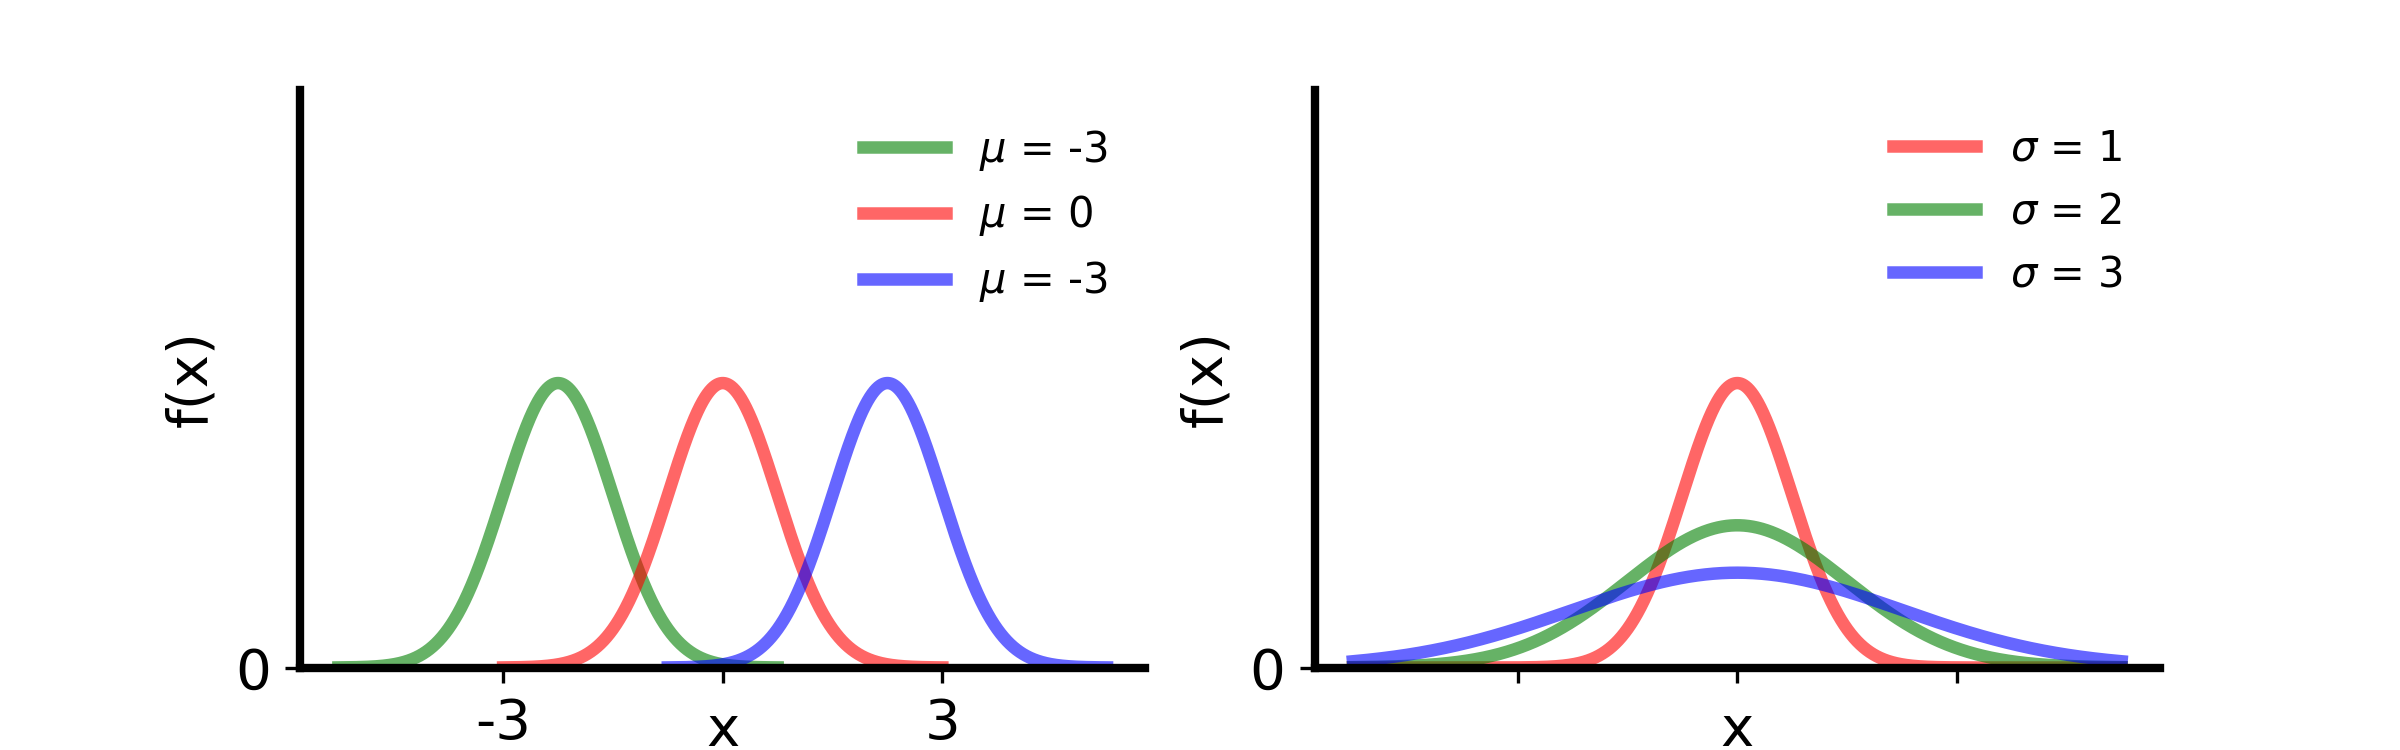
\includegraphics[height=3cm]{images/normal_mu_sig.png}
\end{center}
}

\onslide<3->{
The normal distribution is the most important distribution in all of probability theory. It is ubiquitous in statistical analysis (see central limit theorem). 
}

%\onslide<2->{
%This density function is a bell-shaped curve that is symmetric about $\mu$.
%}

\end{frame}

\begin{frame}
\frametitle{Linear transformation of a normal random variable}

\vspace{-0.2cm}

\begin{claim}
If $X$ is normally distributed with parameters $\mu$ and $\sigma$, then $Y = aX + b$ is normally distributed with parameters $a\mu + b$ and $a\sigma$.
\end{claim}

\onslide<2->{
\begin{proof}
\onslide<2->{
Let $F_Y$ denote the CDF of $Y = a X + b$, then}
\begin{align*}
%F_Y(x) &= P(Y \leq x)\\
\onslide<2->{
F_Y(x) &= P(aX + b \leq x)\\
}
\onslide<3->{
&= P(X \leq (x-b)/a)\\
}
\onslide<4->{
&= F_X((x-b)/a),
}
\end{align*}
\onslide<4->{where $F_X$ is the CDF of $X$. }\onslide<5->{By differentiation, the PDF of $Y$ is
\begin{align*}
f_Y(x) &= \frac{1}{a}f_X((x-b)/a)\\
}
\onslide<6->{
&= \frac{1}{a\sigma \sqrt{2 \pi}} e^{-\frac{1}{2}\big(\frac{\frac{x-b}{a}-\mu}{\sigma}\big)^2}\\
}
\onslide<7->{
&= \frac{1}{a\sigma \sqrt{2 \pi}} e^{-\frac{1}{2}\big(\frac{x-(a\mu+b)}{a\sigma}\big)^2} \qedhere.}
\end{align*}
\vspace{-0.2cm}
\end{proof}
}

\end{frame}

\begin{frame}
\frametitle{The standard normal random variable}

When $X$ is a normal random variable with parameters $\mu$ and $\sigma$, the computation of $P(a \leq X \leq b)$ requires evaluating

\begin{equation*}
\int_a^b \frac{1}{\sigma\sqrt{2 \pi}} e^{-\frac{1}{2}(\frac{x-\mu}{\sigma})^2} dx.
\end{equation*}

\vspace{0.2cm}

\onslide<2->{
This cannot be calculated in closed form. 
}

\vspace{0.2cm}

\onslide<3->{
However, for $\mu = 0$ and $\sigma = 1$, this integral has been approximated and tabulated for certain values of $a$ and $b$. This table can also be used to compute probabilities for any other values of $\mu$ and $\sigma$.
}

\onslide<4->{
\begin{definition}
The normal distribution with parameter values $\mu = 0$ and $\sigma = 1$ is called the \textbf{standard normal distribution}. A random variable $Z$ having a standard normal distribution is called a \textbf{standard normal random variable} and has probability density function given by
\begin{equation*}
f_Z(z; 0, 1) = \frac{1}{\sqrt{2 \pi}} e^{-\frac{1}{2}z^2} .
\end{equation*}
\end{definition}
}

\end{frame}

\begin{frame}
\frametitle{Tabulated CDF of the standard normal distribution}

\begin{center}
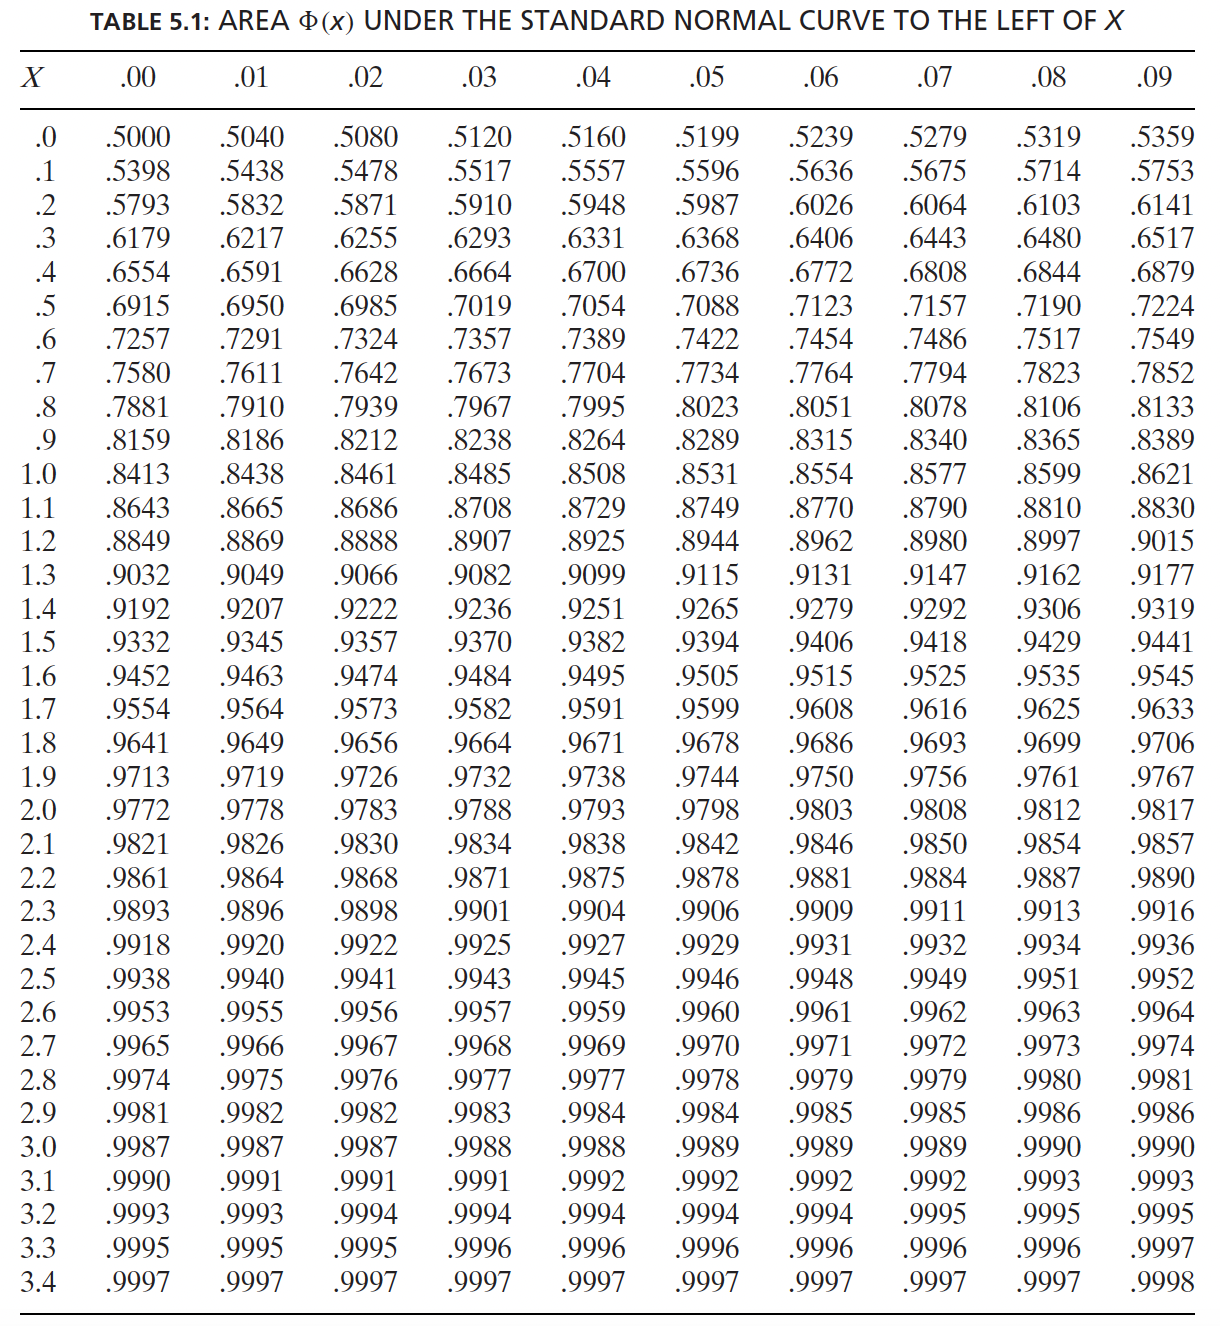
\includegraphics[height=7cm]{images/table.png}
\end{center}

\end{frame}

\begin{frame}
\frametitle{Standardising a normal random variable}

%For a nonstandard normal random variable, when $X \sim \mathcal{N}(\mu, \sigma^2)$, probabilities involving $X$ are computed by standardising. The \textbf{standardised variable} is $(X-\mu)/\sigma$. 

Probabilities involving a nonstandard normal random variable are computed by standardising.

%Subtracting $\mu$ shifts the mean from $\mu$ to 0, and then dividing by $\sigma$ scales the variable so that the standard deviation is 1 rather than $\sigma$.

\onslide<2->{
\begin{proposition}
If $X$ has a normal distribution with mean $\mu$ and standard deviation $\sigma$, then the \textbf{standardised variable} $Z=(X-\mu)/\sigma$ has a standard normal distribution. Thus
\begin{align*}
P(a \leq X \leq b) &= P\Big(\frac{a-\mu}{\sigma} \leq Z \leq \frac{b-\mu}{\sigma}\Big)\\
&= \Phi\Big(\frac{b-\mu}{\sigma}\Big) - \Phi\Big(\frac{a-\mu}{\sigma}\Big),
\end{align*}
where $\Phi$ is the cumulative distribution function of a standard normal random variable.
\end{proposition}
}

\end{frame}

\begin{frame}
\frametitle{Approximating the binomial and Poisson distributions}

The binomial and Poisson distributions are approximately normal for large $n$ or large $\lambda$.

\

\begin{center}
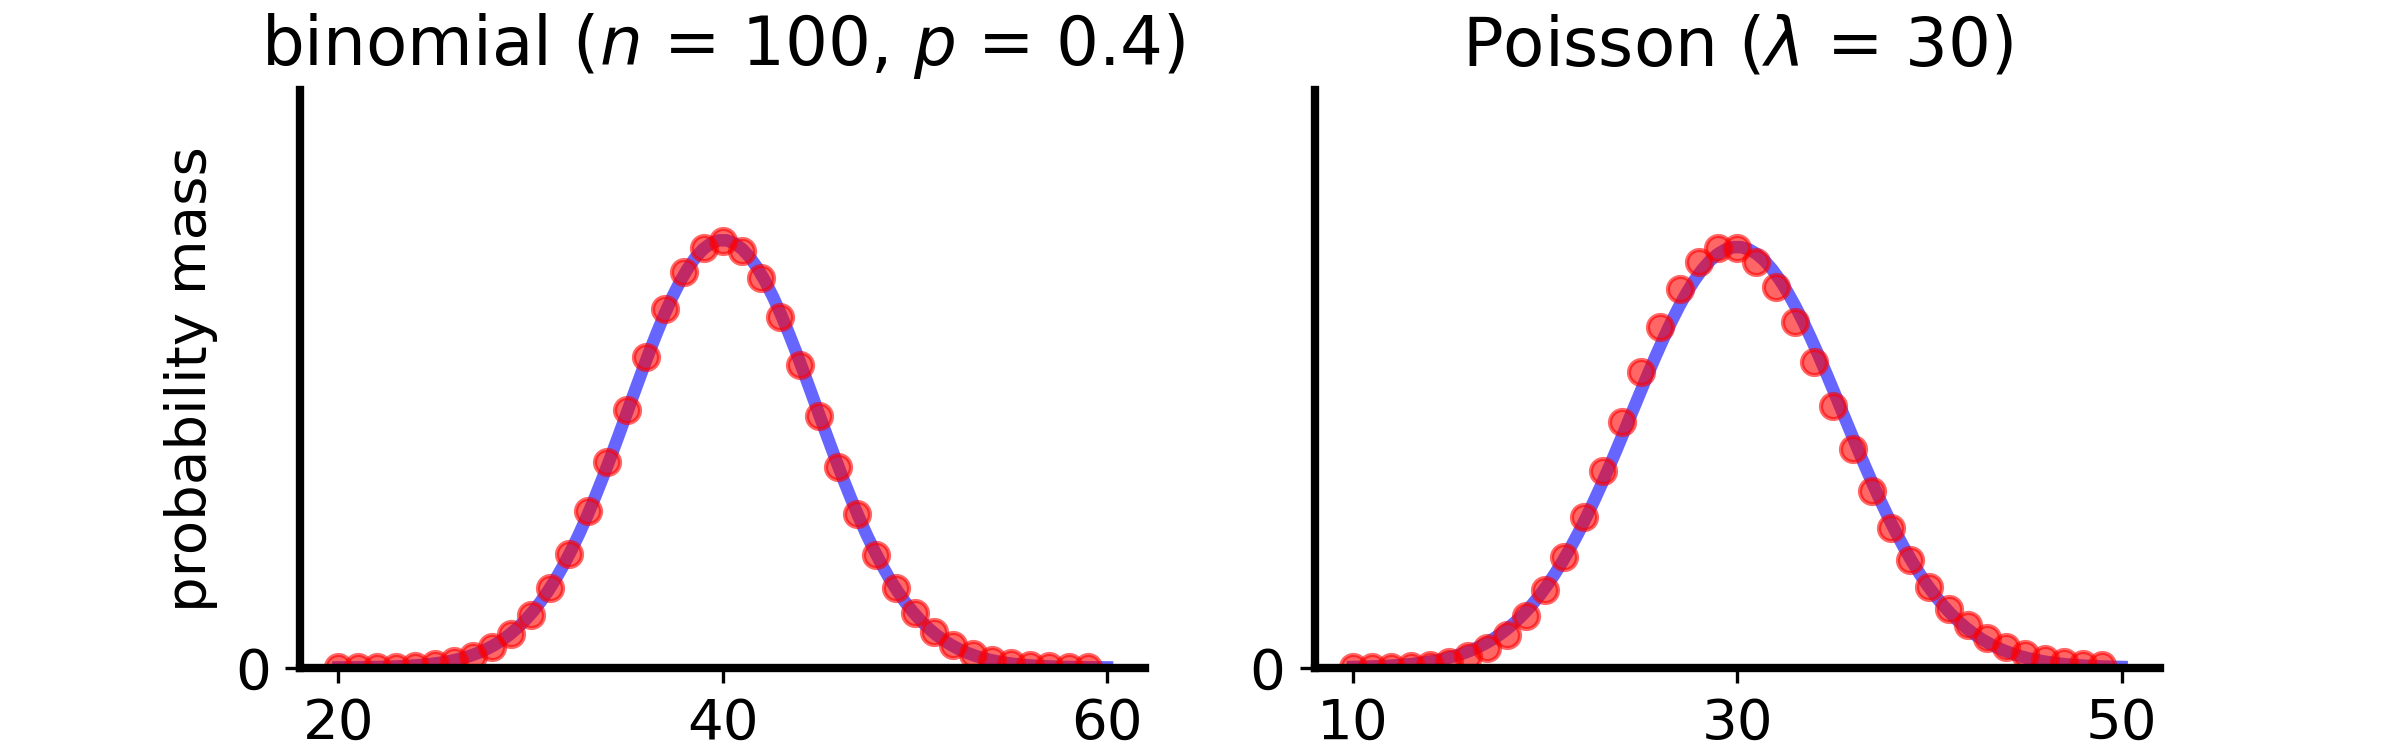
\includegraphics[height=3cm]{images/biniomial_poisson.png}
\end{center}

\onslide<2->{
For the binomial with parameters $n$ and $p$, $\mu = np$ and $\sigma = \sqrt{np(1 - p)}$, and for the Poisson with parameter $\lambda$, $\mu = \lambda$ and $\sigma =\sqrt{\lambda}$.
}

\

\onslide<3->{
These approximations are a great convenience, especially in conjunction with the `$68\%-95\%$ rule'.
}

\end{frame}

\begin{frame}
\frametitle{The exponential distribution: memorylessness}

\begin{theorem}
A random variable $X$ satisfies $X \sim \Exp{\lambda}$ for some $\lambda > 0$ if for all positive $t$ and $h$ the following equation is satisfied:
\begin{equation*}
P(X > t + h | X > t) = P(X > h),
\end{equation*}
that is, if $X$ is memoryless.
\end{theorem}

\onslide<2->{
\begin{proof}
\begin{align*}
\onslide<2->{
P(X > t + h | X > t) &= \frac{P(X > t + h, X > t)}{P(X > t)}\\
}
\onslide<3->{
&= \frac{P(X > t + h)}{P(X > t)}\\
}
\onslide<4->{
&= \frac{e^{- \lambda (t+h)}}{e^{- \lambda t}}\\
}
\onslide<5->{
&= e^{- \lambda h}\\
}
\onslide<6->{
&= P(X > h). \qedhere
}
\end{align*}
\end{proof}
}

%The exponential distributions are the only distributions7 that satisfy Eq. (5.10).

\end{frame}

\section{Summary}
\begin{frame}
\frametitle{Summary}

\begin{enumerate}[label=\textbullet]
    \item Introduced the concept and formal definition of a continuous random variable and a probability density function.
    \onslide<2->{
        \item Learnt how to find the probability that a continuous random variable falls in some interval [a, b].
        }
%        \onslide<3->{
%    \item Learn that if $X$ is continuous, the probability that $X$ takes on any specific value is 0.
%    }
    \onslide<3->{
    \item Introduced the concept and formal definition of a cumulative distribution function of a continuous random variable.
    }
    \onslide<4->{
    \item Learnt how to find the cumulative distribution function of a continuous random variable from the probability density function (and vice versa).
    }
    \onslide<5->{\item Introduced the concept and formal definition of the expected value of a function of a continuous random variable.
    }
     \onslide<6->{\item Learnt how to find the mean and variance of a continuous random variable.
    }
     \onslide<7->{\item Learnt how to sample a continuous random variable using the inverse transform method.
    }
    \onslide<8->{\item Introduced some important probability distributions for a continuous random variable (the uniform, normal and exponential distributions).
    }
\end{enumerate}

\end{frame}


\section{References}
\begin{frame}
\frametitle{References}

%\textbf{References}

This lecture was based on the following textbooks:

\

\begin{enumerate}[label=\arabic*.]
\item Ross, S. (2010). A first course in probability. Pearson.
\item Kass, R. E., Eden, U. T., \& Brown, E. N. (2014). Analysis of neural data (Vol. 491). New York: Springer.
\item Devore, J. L. (2011). Probability and Statistics for Engineering and the Sciences. Cengage learning.
\end{enumerate}

\
 
Problems (with solutions) can be found in Chapter 5 of \href{http://www.gatsby.ucl.ac.uk/~rapela/gcnuBridging2023/books/ross10-aFirstCourseInProbability.pdf}{A first course In probability}.

\end{frame}


% \begin{frame}
% \frametitle{The Dirac delta}
% \end{frame}

% \iffalse 
% CTrl + /
% %\begin{comment}
% %\section{Second section}

% \begin{frame}
% \frametitle{Highlighting text}

% In this slide, some important text will be
% \alert{highlighted} because it's important.
% Please, don't abuse it.

% \begin{block}{Remark}
% Sample text
% \end{block}

% \begin{alertblock}{Important theorem}
% Sample text in red box
% \end{alertblock}

% \begin{examples}
% Sample text in green box. The title of the block is ``Examples".
% \end{examples}
% \end{frame}
% %\end{comment}
% \fi
\end{document}